\documentclass[10pt,a4paper]{report}
%\usepackage[left=1cm,right=1cm,top=1cm,bottom=1cm,bindingoffset=0cm]{geometry}
\usepackage[T2A]{fontenc}
\usepackage[utf8]{inputenc}
\usepackage[russian]{babel}
\usepackage{cmap}
\usepackage{amsmath}
\usepackage{amsfonts}
\usepackage{amssymb} 
\usepackage{hyperref}
\usepackage{stackrel}
\usepackage{graphicx}
%\widetilde
\nonfrenchspacing
\righthyphenmin=2
\def\jo{\"e}
\def\num{\textnumero}

%%%%% Формулы
\def\le{\leqslant} % Делает знак неравенства классическим
\def\ge{\geqslant}
\def\emptyset{\varnothing} % Обычное пустое множество
\def\divisible#1#2{#1\hspace{2.5pt}\raisebox{-1.5pt}{\smash{\vdots}}\hspace{2.5pt}#2}
\def\eqmod#1#2#3{#1\equiv#2\mbox{\hspace{2mm}(mod $#3$)}}
\def\so{\Rightarrow}
\def\theoremend{\hfill\vbox to 0pt{\hbox{$\square$}}}
\def\solutionend{\hfill$\blacksquare$}
\def\quest#1{\stackrel{?}{#1}}
\def\epsilon{\varepsilon}
\def\phi{\varphi}
\def\rddots#1{\cdot^{\cdot^{\cdot^{#1}}}} % Зеркальное отражение \ddots
%\def\modop{\ \ \mbox{mod}\ \ }

\def\missing{\rule[-0.33em]{1em}{1.36em}\fbox{???}\rule[-0.33em]{1em}{1.36em}}
\def\missingwhat#1{\fbox{\parbox{10cm}{#1}}}


\def\df{{\bfseries Определение. }}
\def\pr#1{{\bf Задача \num#1. }}
\def\th{{\bfseries Теорема. }}
\def\bigmid{\mathrel{}\middle|\mathrel{}}
\def\solutionstart{$\square$\;\;}
\def\therm#1{{\it #1}}

\usepackage{indentfirst}
\DeclareMathOperator{\Mat}{Mat}
\DeclareMathOperator{\M}{M}
\DeclareMathOperator{\Sp}{Sp}
\DeclareMathOperator{\Tr}{Tr}
\DeclareMathOperator{\tr}{tr}
\DeclareMathOperator{\Def}{def}
\DeclareMathOperator{\id}{id}
\DeclareMathOperator{\odd}{odd}
\DeclareMathOperator{\Det}{Det}
\DeclareMathOperator{\Vol}{Vol}
\DeclareMathOperator{\sign}{sign}
\DeclareMathOperator{\sgn}{sgn}
\DeclareMathOperator{\Id}{Id}
\DeclareMathOperator{\ord}{ord}
\DeclareMathOperator{\adj}{adj}
\DeclareMathOperator{\rk}{rk}
\DeclareMathOperator{\re}{Re}
\DeclareMathOperator{\Ker}{Ker}
\DeclareMathOperator{\im}{Im}
\DeclareMathOperator{\Arg}{Arg}
%\DeclareMathOperator{\ch}{ch}
%\DeclareMathOperator{\ker}{ker}
\DeclareMathOperator{\Rg}{Rg}
\DeclareMathOperator{\Dom}{Dom}
\DeclareMathOperator{\diag}{diag}
\DeclareMathOperator{\Gr}{Gr}
\DeclareMathOperator{\Tor}{Tor}
\DeclareMathOperator{\ort}{ort}
\DeclareMathOperator{\PR}{pr}
\DeclareMathOperator{\grad}{grad}
\DeclareMathOperator{\rank}{rank}
\DeclareMathOperator{\Char}{char}
\DeclareMathOperator{\Int}{int}
\DeclareMathOperator{\Ext}{ext}
\DeclareMathOperator{\diam}{diam}
\DeclareMathOperator{\cov}{cov}
\DeclareMathOperator{\dom}{dom}

\def\deflr{\stackrel[\Def]{}{\Longleftrightarrow}}

\def\dvec#1#2{\begin{pmatrix}
#1\\#2
\end{pmatrix}}
\def\ov#1{\overrightarrow{#1}}
\def\ovl#1{\overline{#1}}
\def\mat#1#2#3{\begin{pmatrix}
#1_{11} & #1_{12} & \ldots & #1_{1#3}\\
\vdots &  & \ddots & \vdots \\
#1_{#2 1} & #1_{#2 2} & \ldots & #1_{#2#3}
\end{pmatrix}
}
\def\vec#1#2{\left(\begin{smallmatrix}#1\\\vdots\\
#2\end{smallmatrix}\right)}
\def\system#1#2{\left\{
\begin{aligned}
#1\\
\vdots\\
#2\\
\end{aligned}
\right.
}
\def\blockmatrix#1#2#3#4{\left(
\begin{array}{c|c}
  #1 & #2 \\ \hline
  #3 & #4
\end{array}
\right)}


\def\Uc{\stackrel{\circ}{U}}
\def\rra#1{\stackrel{#1}{\rightrightarrows}}
\def\E{\mathbb E}
\def\D{D}
\def\vrt#1{\left\lVert#1\right\rVert}
\def\br#1{\left(#1\right)}
\def\brc#1{\left\{#1\right\}}
\def\abs#1{\left|#1\right|}
% \stackrel stackbin 

\usepackage{setspace}
\begin{document}
\setstretch{1.4}

\thispagestyle{empty}
\begin{center}
  Правительство Российской Федерации\\
  Федеральное государственное автономное образовательное\\
  учреждение высшего образования\\
  <<Национальный исследовательский университет\\
  <<Высшая школа экономики>>\\[1cm]
  Факультет компьютерных наук\\
  Основная образовательная программа\\
  Прикладная математика и информатика\\[2cm]
\bfseries
  {\large ВЫПУСКНАЯ КВАЛИФИКАЦИОННАЯ РАБОТА}\\
  на тему\\
  <<Разработка компоненты интерактивной визуализации графа совстречаемости терминов для информационной системы iFORA>>\\[1cm]
\end{center}
\mdseries
\begin{flushright}
  Выполнил студент\\
  группы БМПИ144, 4 курса,\\
  Сергиенко Ярослав Михайлович\\[1cm]

  Научный руководитель:\\
  доцент, старший научный сотрудник,\\
  Незнанов Алексей Андреевич\\[1cm]

  Консультант:\\
  зав. отделом информационно-аналитических\\
  систем ИСИЭЗ, к.г.н.,\\
  Кузьминов Илья Филиппович \\

\end{flushright}
\vfill
\centerline{Москва 2018}
\newpage

\tableofcontents

\newpage

Ключевые слова: t-SNE, Barnes-Hut optimization, Fruchterman Reingold, WebGL computations, video visualization, single-page web application.

\section*{Введение}
\label{sec:intro}
\addcontentsline{toc}{section}{\nameref{sec:intro}}

Обычно при проектировании веб-приложений существует стандартное разделение ответственности между браузером клиента и сервером. Cерверу доступно больше ядер процессора и оперативной памяти, чем клиенту. К тому же браузер не имеет доступа к жесткому диску, так что любые сложные вычисления лучше производить на стороне сервера и передавать результат клиенту.

К 2014 году в большинстве браузеров появился доступ к упрощенному API графических карт благодаря технологии WebGL. С учетом того, что у большинства серверов отсутствует графическая карта, некоторые виды вычислений могут значительно быстрее выполняться на стороне клиента.

Данная работа посвящена созданию экспериментального (но решающего реальную задачу) веб-приложения, которое выигрывает от использования графической карты двумя различными способами. В первой главе приводится описание задачи, требования к приложению и его архитектура.

Вторая глава посвящена общим вычислениям на графической карте. Обсуждаются, почему не все алгоритмы, которые могут эффективно вычисляться на графической карте (например, в CUDA), могут так же эффективно вычисляться с использованием довольно ограниченного WebGL API. {\bfseries Впервые} приводится обоснование возможности и псевдокод реализации эффективного (то есть с использованием ряда оптимизаций, включая Barnes-Hut) вычисления t-SNE на шейдерах WebGL. Производятся замеры производительности, показывающие увеличение производительности реализации стандартной (то есть без оптимизаций) версии t-SNE в десятки раз при использовании шейдеров WebGL по сравнению со стандартной (без оптимизаций) реализацией на языке C.

Третья глава посвящена генерации графики при помощи графических карт. Обсуждается сложность разработки интерактивных трехмерных визуализаций и генерации качественного видео на их основе. Предлагается формат хранения интерактивных визуализаций, который может быть воспроизведен при помощи небольшого веб-приложения. Это же приложение может работать как рендер-ферма для создания высококачественного видео на основе такого же файла. Приводится реализация четерых стандартных методов пост-обработки, включенных в профессиональные программы наподобие Adobe After Effects.
\\
\\
Исходный код приложения доступен по адресу\\
\url{https://github.com/pallada-92/text-graph}\\
\\
Предварительная видео-визуализация доступна по ссылке\\
\url{https://www.youtube.com/watch?v=D3DHO_ovXf0}\\
\\
Пример видео с пост-обработкой доступен по ссылке\\
\url{https://youtu.be/sPLuj1rHljY}\\

\section*{Обзор литературы}
\label{sec:lit_review}
\addcontentsline{toc}{section}{\nameref{sec:lit_review}}

Задача интерактивной визуализации графа совстречаемости терминов при помощи WebGL лежит на стыке нескольких областей, по каждой из которых можно найти множество релевантных публикаций.

Есть две классические статьи 1991 года, которые показали полезность трехмерных визуаизаций: \cite{classic_ecologies} показывает изменение древовидной структуры во времени, \cite{classic_3d_trees} позволяет интерактивно перемещаться по иерархической стркутуре.

В некоторых статьях описываются общие решения, которые могут быть полезны при проектировании приложений для интерактивного анализа данных. В статье \cite{interactive_coordinated_views} показана техника coordinated views, позволяющая использовать несколько окон для отображения связанной информации. Статья \cite{25d_vislink} представляет механизм VisLink для соотнесения одних и тех же объектов на разных плоских визуализациях в трехмерном пространстве. В статье \cite{in_situ} приводится сложная в реализации, но очень мощная техника In Situ Exploration, позволяющая переходить плавно переходить между визуализациями связанных данных в зависимости от контекста.

Есть примеры успешной реализации интерактивных веб-приложений для анализа данных. Описание (на данный момент устаревшей) архитекруты системы для интерактивной визуализации графов приводится в \cite{scalable_web}. Интерактивный анализ текстов затронут в \cite{interactive_document_exploration}. Интерактивная визуализация графов рассматривается в статьях \cite{interactive_relations}, \cite{interactive_large_graph}, \cite{interactive_tpp}. Интерактивные трехмерные графы появляются в статьях \cite{interactive_3d_graph}, \cite{interactive_graph_3d_fast}, \cite{graph_interactive}.

Как оказалось, часто наиболее информативные трехмерные визуализации состоят из нескольких плоских визуализаций. Эта техника называется 2.5D. Статьи \cite{25d_simultaneous} и \cite{25d_interactive_graph} использует 2.5D для соотнесения графов во времени, при этом в последней используются интерактивные визуализации. В \cite{25d_bloggers} представлена визуализация 2.5D, показывающая изменения во времени в коллекции текстовых документов. 

Множество статей посвящены оптимизации рисования больших графов: в биоогии \cite{bio_graph}, в анализе текстов \cite{large_document}, для интерактивных визуализаций \cite{interactive_large_graph}. Общий обзор средств дан в статье \cite{large_graph_survey}.

При реализации t-SNE использовалась оригинальная статья \cite{tsne} с оптимизациями, описанными в \cite{acc_tsne}. Оригинальная идея Barnes-Hut simulation была описана в статье \cite{barnes_hut}.

При использовании модели word2vec было необходимо рассчитать размер надписи термина на основании его абсолютной встречаемости и длины вектора. Подробное изучение связи этих трех величин было проведено в статье \cite{v2w_length}.

Хороший обзор алгоритмов force-directed drawing дан в учебниках \cite{book_graph_drawing} и \cite{book_force}. Использовалась также оригинальная статья по алгоритму Fruchterman Reingold \cite{fr}.

%\section*{Выводы}
%\label{sec:lit_concl}
%\addcontentsline{toc}{section}{\nameref{sec:lit_concl}}

\chapter{Архитектура приложения}

\section{Описание существующей системы}

Институт статистических исследований и экономики знаний (ИСИЭЗ) является крупным подразделением НИУ ВШЭ, занимающийся исследованиями в области статистики науки, технологий, инноваций, образования и подготовки кадров, информационного общества и цифровой экономики, научно-технической и инновационной политики.

iFORA (intelligent foresight analytics) является одной из множества информационных систем института, специализирующаяся на майнинге массива научных публикаций, патентов, грантов, специализированных медиа и других документов. Она обладает множеством возможностей, включая:

\begin{itemize}
\item Выделение именных сущностей, ключевых слов и словосочетаний. Определение канонической формы сущностей, сопоставление с онтологической базой (например, DBPedia).
\item Поиск по инвертированному индексу, поддержка сложных поисковых запросов.
\item Обученные \texttt{word2vec} модели на различных выборках текстов.
\item Непрерывное пополнение данных из различных источников включая платные базы, открытые ресурсы и веб. При необходисти используются парсеры.
\item Проверка и редактирование данных экспертами в полуручном режиме.
\item Возможность получить выгрузку по поисковому запросу с множеством настроек в виде архива, содержащего векторные файлы с диаграммами и визуализациями, .rds-файлы с данными (бинарный формат представления табличных данных в R) и автоматически сгенерированную заготовку презентации.
\end{itemize}

\section{Содержание выгружаемых данных}

Взаимодействие с существующей системой происходило через получение выгрузки определенного формата.

Выгрузка по поисковому запросу содержала:

\begin{itemize}
\item Несколько тысяч именованных сущностей, их встречаемость, центральность, специфичность, разбиение на кластеры методом {\itshape Louvain Modularity} \cite{communities}.
\item Встречаемость сущностей по годам.
\item Совстречаемость сущностей по годам. При построении графа совстречаемости использовались не все найденные документы, а окрестности найденных ключевых слов, что увеличивало релевантность получающегося графа.
\item Для каждого года общее количество обработанных документов.
\end{itemize}

Также для разичных выборок документов были доступны обученные word2vec модели из векторов размерности 200, содержащие порядка нескольких миллионов сущностей.

\section{Техническое задание}

Данный проект является результатом эксперимента по совершенствованию текущих и добавлению новых видов интерактивных визуализаций в браузере:
\begin{itemize}
\item Базовая функциональность:
  \begin{itemize}
  \item Возможность просмотра двумерной визуализации графа совстречаемости терминов.
  \item Изменение масштаба, перемещение при помощи мыши.
  \item Цвет надписей соответствует кластерам.
  \item Размер надписей зависит от их центральности.
  \item Если две надписи перекрываются, показывается более центральная. При увеличении показывается больше надписей.
  \end{itemize}

\item Семантическая карта:
  \begin{itemize}
  \item Нанесение терминов на двумерную карту с заданными осями, например, частота $\times$ специфичность.
  \item Возможность просмотра двумерной карты терминов, построенной применением алгоритма t-SNE к модели word2vec.
  \end{itemize}

\item Автономная работа:
  \begin{itemize}
  \item Все приложение содержится в одном html-файле, при помещении которого в папку с выгрузкой есть возможность просматривать визуализации без сервера.
  \item Возможность сгенерировать визуализацию при помощи сервера, сохранить её в файл и открыть позже без сервера.
  \end{itemize}

\item Поиск:
  \begin{itemize}
  \item Строка поиска для быстрого перемещения к ключевому слову.
  \item Поисковые подсказки при наборе слова.
  \item Поиск семантически похожих слов по модели word2vec.
  \end{itemize}

\item Время:
  \begin{itemize}
  \item Возможность просмотра графа совстречаемости по годам.
  \item При переходе между годами граф плавно перестраивается, отражая изменения частот совстречаемости.
  \end{itemize}

\item Интерактивность:
  \begin{itemize}
  \item При нажатии по термину камера центрируется на нем.
  \item При наведении мыши на термин появляется всплывающая подсказка с дополнительной информацией.
  \item Возможность сохранения текущих параметров камеры в виде ссылки.
  \end{itemize}

\item Трехмерные визуализации:
  \begin{itemize}
  \item Вращение камеры, изменение масштаба.
  \item Просмотр двумерного графа совстречаемости или семантической карты с добавленной третьей координатой, например, центральность.
  \item Просмотр трехмерной визуализации word2vec при помощи t-SNE.
  \item Просмотр трехмерной визуализации графа совстречаемости.
  \end{itemize}

\item Видео-визуализации:
  \begin{itemize}
  \item Сохранение и просмотр анимированных визуализаций.
  \item Экспорт анимированной визуализации в виде видео.
  \end{itemize}
\end{itemize}

\section{Автономная работа}

Требование автономной работы было добавлено по нескольким причинам. Во-первых, в целях безопасности сервера iFORA размещались в локальной сети и могли быть недоступны во время презентации вне ВШЭ. Во-вторых, это упрощало поддержку и внедрение системы. В-третьих, это экономило ресурсы и переносило нагрузку с серверов на браузер пользователя.

Для автономной работы было необходимо реализовать некоторые алгоритмы визуализации данных в браузере. Было решено использовать Fruchterman-Reingold для графов совстречаемости и t-SNE для семантических карт word2vec представлений терминов.

Оба алгоритма имели множество реализаций (вкючая оптимизации типа Barnes-Hut \cite{barnes_hut}) на JavaScript. Однако эти реализации очень медленно работали на нескольких тысячах вершин. Так как использование графической карты потенциально могло ускорить эти алгоритмы и так как не было реализаций с использованием GPU, было принято решение провести эксперимент по портированию алгоритмов для вычислений в шейдерах WebGL.

\section{Производительные вычисления в браузере}

До недавнего времени, единственным языком программирования, доступным в большинстве браузеров, являлся язык JavaScript. С момента своего появления в 1995 году и до 2015 года, он претерпевал незначительные изменения. Со второй половины 2000-х годов стали набирать популярность {\itshape одностраничные веб-приложения}, которые выполняли часть работы сервера (в основном, связанную с генерацией html-кода) на стороне клиента.

В 2008 году Google выпускает браузер Chrome с новым Javascript-движком V8, который значительно превосходил другие реализации по производительности за счет встроенного JIT-компилятора. Сложность его реализации состояла в том, что JavaScript создавался как интерпретируемый, динамически типизируемый язык.

После 2010 года появляются несколько экспериментальных технологий, которые были направлены на улучшение производительности:

\begin{itemize}
\item {\bfseries Typed Arrays} (2010) --- возможность языка, позволяющая создавать {\itshape типизированные массивы}, для которых можно было определять двоичное представление в памяти.
\item {\bfseries WebGL} (2010) предоставил доступ к API графической карты схожий с OpenGL ES 2.0.
\item {\bfseries asm.js} (2013) --- подмножество языка JavaScript, которое по семантике схоже с виртуальной машиной, используемой JIT-компиятором, что позволяло писать низкоуровневый код по производительности не уступающим аналогичному коду на \texttt{C}. В нем ручное управление памятью, что позволило отказаться от сборщика мусора. Также, в отличие от обычного кода, у всех переменных в \texttt{asm.js} присутствует информация об их типах, что позволяет компилировать код перед выполнением, а не динамически.
\item {\bfseries WebCL} (2014) должен был предоставить возможность выполнения OpenCL вычислений в браузере, что должно было решить большую часть проблем, решаемых в данной главе, но так и не был включен в стандартную поставку ни одного из популярных браузеров.
\item {\bfseries Service Workers} (2015) позволяют создавать дополнительные потоки, которые выполняются параллельно с основным кодом. Таким образом, сложные вычисления могли происходить в фоновом режиме и не влиять на отзывчивость интерфейса.
\item {\bfseries WebAssembly} (2017) является логическим продолжением \texttt{asm.js}, позволяя передавать в браузер непосредственно байт-код виртуальной машины. По сравнению с \texttt{asm.js}, имеет меньший размер, не требует синтаксического разбора, обладает большим набором команд и может быть целевой архитектурой компилятора LLVM, т.е. позволяет компилировать код с любого другого языка без потери производительности.
\end{itemize}

В данной работе используются только первые три технологии. Было установлено, что использование GPU значительно замедляет работу всей системы, независимо от того, происходит это в основном потоке или в service worker. Также оказалось, что для рассматриваемых алгоритмов \texttt{asm.js} показывает такой же результат, что и код на обычном JavaScript (и сравнимый с нативным кодом). Так как данная работа фокусируется на ускорении основного цикла алгоритмов при помощи GPU, было принято решение не использовать WebAssembly, преимущество которого состоит, в первую очередь, в быстром запуске кода и портировании с других языков для исполнения на CPU.

\section{Решение проблемы возрастающей сложности разработки}

Во время работы над техническим заданием возникла проблема, заключающаяся в том, что было необходимо создать, с одной стороны, средство генерации качественных интерактивных визуализаций, с другой --- простое в использовании и разработке веб-приложение. При этом должна быть возможность быстрого добавления и проверки экспериментальных функций.

Другая проблема состояла в том, что все данные невозможно было обрабатывать в браузере (например, выгрузка word2vec занимала больше гигабайта), следовательно, было необходимо создавать логику предобработки данных на сервере. При этом нельзя было все вычисления производить на сервере, т.к. тогда визуализации перестанут быть интерактивными. Если же логика обработки данных разделена между сервером и приложением, появляется сложное API их взаимодействия. При этом добавление новой функции требует изменения как со стороны сервера, так и со стороны клиента, что многократно увеличивает время разработки и делает невозможным быстрое внедрение новых фукнций.

Также было замечено, что прототипирование на языке python в среде типа Jupyter происходит быстрее всего, т.к. в нем доступно больше всего библиотек анализа и обработки данных, можно быстро сохранять и загружать промежуточные результаты в виде файлов. При работе в аналогичных средах для Javascript (например, Observable.JS) размер документа, в котором можно комфортно работать, гораздо меньше.

В итоге было принято решение перенести всю логику создания интерактивных визуализаций на сторону сервера и разработать такой формат их хранения, который:
\begin{itemize}
\item При добавлении новых видов визуализаций не требуется вносить изменения в формат.
\item Самодостаточен, то есть содержит в себе все необходимые данные.
\item При создании нескольких визуализаций с общими данными, должна быть возможность избежать их копирования.
\item Не содержит кода на JavaScript.
\item Эффективен по производительности.
\item Визуализации меняются во времени и, возможно, имеют настраиваемые параметры.
\item Работает на большинстве ПК, мобильных устройств и планшетов.
\item Поддерживает рендер видео с использованием пост-эффектов: прозрачность, motion blur, lens blur, antialiasing и любых других.
\end{itemize}
Тогда приложение является всего лишь <<проигрывателем>> таких файлов. Разработка ведется на любом языке программирования (например, python) при необходимости через браузер записывается видео.

Этот формат также решает проблему автономной работы приложения: достаточно сохранить файл с визуализацией.

Недостаток такой схемы состоит в том, что для генерации визуализаций требуется делать запрос к программисту, в то время как обычный пользователь не имеет возможности создавать визуализации автоматически.

Решение состоит в том, чтобы часто используемый код перенести на отдельный сервер, который будет генерировать файл с визуализацией. В случае, если необходимо генерировать визуализации интерактивно, можно создать отдельное веб-приложение для этого и встроить в него <<проигрыватель>>.

Такое разделение позволяет добавлять новые виды визуализаций, не усложняя приложение и серверную часть.

\section{Сравнение с аналогами}

Приложение в первую очередь сравнимо с такими продуктами как Gephi и Tensorflow Embedding Projector. Несмотря на гораздо меньшую функциональность с точки зрения пользователя, это приложение имеет следующие преимущества: возможность быстрого прототипирования и воспроизведения разнообразных визуализаций, сохранение анимаций в видео, гораздо более быстрое выполнение алгоритмов t-SNE и force-directed graph drawing.

\chapter{Алгоритмы визуализации данных в браузере}

В данной главе описываются реализации двух алгоритмов визуализации данных: Fruchterman Reingold и t-SNE.

Несмотря на наличие множества реализаций этих алгоритмов на JavaScript, ни одна из них не использует GPU. При этом нет простого способа портировать существующие реализации этих алгоритмов на GPU с других языков программирования, так как WebGL API очень ограничен по сравнению с OpenGL и другими API для графических карт.

\section{WebGL для обработки данных}
\label{sec:webgl_data_analysis}

С середины 2000-х графические карты активно используются для научных вычислений. С ростом популярности глубинного обучения инструменты для вычислений на GPU вошли в стандартный набор специалистов по анализу данных: OpenCL, CUDA, Tensorflow и другие.

Появление WebGL сделало возможным вычисления с использованием GPU в браузере. Есть несколько специализированных библиотек для JavaScript, например: tensorflow.js, gpu.js, turbo.js. В первую очередь они используются для глубинного обучения и операций с матрицами. Идея gpu.js состоит в трансляции кода с JavaScript в язык шейдеров.

Проблема технологии WebGL для обработки данных состоит в том, что она предлагает очень ограниченный набор возможностей по сравнению, например, с CUDA. С другой стороны, это сделало возможным его поддержку 98\% устройств, включая смартфоны, планшеты и игровые приставки. Существует также несколько расширений WebGL, которые поддерживаются не всеми устройствами. Наконец, существует стандарт WebGL 2, в котором множество расширений включено по умолчанию, но он на данный момент поддерживается только 43\% устройств.

Вычислительная модель WebGL основана на двух сущностях: текстуры и шейдеры. Упрощенно, на первом этапе строится трехмерная полигональная модель сцены, затем строится её двумерная проекция и ко всем пикселям проекции каждого объекта могут быть применены шейдеры. При обработке данных, обычно строится единственный треугольник, занимающий всю проекцию и к нему применяется единственный шейдер. Таким образом, шейдер --- это функция, независимо применяемая для каждого пикселя (также называемых {\itshape текселями}) получающегося в результате изображения.

На вход шейдер принимает набор {\itshape аттрибутов}, которые для трехмерных сцен могут кодировать нормали или текстурные координаты. При обработке данных аттрибуты не используются и шейдер имеет лишь координаты текущего пикселя.

Шейдеру также доступен набор глобальных констант ({\itshape uniforms}), которые могут быть квадратными вещественными матрицами или векторами размерности не более 4, а также текстурами. Для текстуры шейдер может получать значение любого пикселя. То есть, чтобы шейдер мог обрабатывать данные, их необходимо закодировать в виде текстуры.

\section{Текстуры для хранения данных в WebGL}

Результат работы шейдера может быть выведен на экран, а может быть сохранен в текстуру. Полученная текстура может быть использована другими шейдерами, а также может быть передана на процессор. Передача текстур между CPU и GPU является дорогой операцией и может занимать до половины времени выполнения программы.

Текстуры бывают разных типов: RGBA, RGB, целые или вещественные 16- или 32-битные. Для поддержки числовых текстур требуются расширения, но такие текстуры не могут передаваться от GPU к CPU, что значительно уменьшает их полезность. Таким образом, основным способом хранения данных являются RGBA текстуры.

RGBA текстуры представлены как массив 32-битных чисел, состоящих из 4 компонент, принимающих значения от 0 до 255. За одно обращение шейдер получает один пиксель текстуры, явяющийся вектором из четырех 8-битных чисел. Таким образом, без использования расширений в пикселях текстуры можно закодировать целые 32-битные значения или два 16-битных.

При обработке данных серъезной проблемой является ограничение на то, что шейдер может вернуть результат лишь в виде одного 32-битного числа. Если, например, шейдер работает с трехмерными точками, то потребуется либо возвращать каждую компоненту по отдельности, то есть повторять одни и те же вычисления три раза, либо кодировать положение точки в 32-битное число, что значительно ухудшит точность. Поэтому в данной работе используется расширение \texttt{WEBGL\_draw\_buffers}, позволяющее подключать от 1 до 4 текстур одного размера к одному шейдеру. В итоге, результатом работы шейдера могут быть от одного до четырех 32-битных чисел. Это расширение поддерживается только 76\% ПК и практически не поддерживается в смартфонах и планшетах.

\section{Ограничения на циклы и условия в шейдерах WebGL}

Помимо перечисленных выше, в WebGL есть еще два существенных ограничения.

Графические карты имеют иерархическую модель выполнения команд, которая может быть доступна в таких языках, как CUDA. Это позволяет обрабатывать множество пикселей одновременно. Проблема состоит в том, что при этом всем обработчикам поступают одни и те же команды. Выполнение условных конструкций достигается временным отключением обработчиков тех пикселей, для которых условие не выполняется. То есть, если в коде есть условие и одна половина пикселей должна выполнить один код, а вторая --- другой, то суммарное затраченое время будет пропорционально сумме, а не минимуму.

Из этого также следует, что если для каждого пикселя необходимо выполнить цикл, то число выполненных итераций будет равно максимуму по всем пикселям. Операция \texttt{break} будет работать корректно, однако затраченное время будет пропорционально верхней оценке, то есть остальные итерации будут выполнены в отключенном состоянии.

Более того, в WebGL при объявлении циклов требуется, чтобы число итераций было константой {\bfseries времени компиляции}. Похоже, что это самое сильное ограничение, возникающее при обработке данных в шейдерах.

Продвинутые графические карты способны определять момент, когда циклы для всех пикселей были остановлены командой \texttt{break}, чтобы уменьшить время выполнения. Это позволяет во время компиляции указать любую большую константу в качестве числа итераций цикла и выйти из него принудительно. Тем не менее, было бы некорректно предполагать наличие этой функциональности у всех пользователей при рассчете сложности алгоритма.

\section{Fruchterman Reingold}

Это классический алгоритм рисования графа из категории force-directed drawing.

Он использует физическую аналогию, в которой ребрам соответствуют пружины, а вершинам --- одинаково заряженные частицы. Таким образом, соединенные ребром вершины стремятся быть на фиксированном расстоянии друг от друга, равном оптимальной длине пружины, а не соединенные вершины отталкиваются друг от друга.

На практике, закон Гука для силы пружины не используется, так как он слишком сильно действует на соединенные вершины, находящиеся в разных частях графа.

Для алгоритма Fruchterman Reingold силы притяжения и отталкивания равны $f_a(d) = d^2 / k$ и $f_r(d) = -k^2 / d$, где $k$ --- оптимальная длина пружины, при которой эти силы сбалансированы.

Обычно, физическая симуляция осуществляется при помощи интегрирования Верле, но в этом алгоритме силы по сути являются скоростями, так как это ускоряет сходимость.

Алгоритм начинает со случайных позиций вершин и останавливается, когда система достигает равновесия. Для ускорения этого процесса вводится понятие {\itshape температуры}, которая ограничивает максимальное изменение положения вершин и уменьшается по заданному закону.

\section{t-SNE}

Применение этого алгоритма считается одним из наиболее мощных методов уменьшения размерности до 1-3 измерений.

В базовой версии он получает на вход множество точек $\brc{x_i}$ в пространстве большой размерности (например, 50), а также начальное случайное положение представлений этих точек $\brc{y_i}$ в пространстве размерности 1-3. Для точек $x_i$ предрассчитывается матрица расстояний $\br{p_{ij}}$ по формуле:

$$p_{ij} = \frac{p_{i|j} + p_{j|i}}{2}$$

\begin{equation}
  p_{j|i} = \frac{\exp(-\vrt{x_i - x_j}^2 / 2 \sigma_i^2)}{\sum_{k\neq i}\exp(-\vrt{x_i - x_k}^2 / 2 \sigma_i^2)},\quad p_{i|i} = 0
  \label{eq:p_conditional}
\end{equation}
где $\sigma_i$ подбираются при помощи двоичного поиска так, чтобы для всех $i$:
$$-\sum_j p_{j|i} \log_2 p_{j|i} = \log_2(\mbox{\itshape perplexity}),$$
где {\itshape perplexity} является параметром алгоритма.

Описанные выше вычисления производятся один раз при инициализации алгоритма. Далее происходят итерации, на каждой из которых вычисляется матрица $\br{q_{ij}}$:

$$ q_{ij} = \frac{(1 + \vrt{y_i - y_j}^2)^{-1}}{\sum_{k\neq l}(1 + \vrt{y_k - y_l}^2)^{-1}},\quad q_{ii} = 0$$
после чего для каждой вершины $y_i$ считается градиент целевой функции:

$$\Delta y_i = 4 \sum_{j\neq i} (p_{ij} - q_{ij}) (y_i - y_j) (1 + \vrt{y_i - y_j}^2)^{-1},$$
на основании чего считаются новые положения $y_i$ и итерация повторияется. При вычислении новых положений предлагается использовать {\itshape momentum term}:
$$y_i^{t} = y_i^{t - 1} + \eta \Delta y_i + \alpha(t)(y_i^{t - 1} - y_i^{t - 2}),$$
где $\eta$ --- фиксированная константа, $\alpha(t)$ --- убывающая функция, $y_i^t$ --- значение $y_i$ после итерации $t$.

\section{Модификации t-SNE для ускорения вычислений}

Данная глава основана на работе \cite{acc_tsne}.

Для вычислений значений $p_{i|j}$ используется нормальное распределение, которое, как известно, при больших отклонениях от центра убывает экспоненциально. Таким образом, можно заменить такие значения на нули.

Смысл параметра {\itshape perplexity} состоит в том, что он является аналогом числа соседей, когда веса ребер являются вероятностями. Это позволяет сделать предположение о том, что среди чисел $p_{i|j}$ число ненулевых членов в каждой строке пропорционально {\itshape perplexity}. Обозначим коэффициент пропорциональности через $c$.

После симметризации, матрица $p_{ij} = (p_{i|j} + p_{j|i}) / 2$ будет иметь не более, чем в два раза больше ненулевых клеток. Ей будет соответствовать граф, в котором из каждой вершины выходит не более $2 c \cdot \mbox{\itshape perplexity}$ ребер.

Заметим, что в формуле $q_{ij}$ знаменатель не зависит от $i$ и $j$ и равен сумме числителей по всем $i$ и $j$. Обозначим его $Z$:
$$Z = \sum_{k\neq l} (1 + \vrt{y_k - y_l}^2)^{-1}, \quad q_{ij} =\frac{(1 + \vrt{y_i - y_j}^2)^{-1}}{Z} $$

Следующая идея состоит в том, чтобы разбить $\Delta y_i$ на два слагаемых:
$$\Delta y_i = 4 \sum_{j\neq i} (p_{ij} - q_{ij}) (y_i - y_j) (1 + \vrt{y_i - y_j}^2)^{-1} = 4 \sum_j (p_{ij} - q_{ij}) (y_i - y_j) q_{ij} Z = $$
$$ = 4\sum_{j\neq i}(p_{ij}q_{ij} - q_{ij}^2)Z(y_i - y_j)$$
Получаем, что между точками $y_{i}$ действует две силы:
\begin{itemize}
\item {\bfseries Сила притяжения}, пропорциональная $p_{ij}q_{ij}$, которая действует только между точками, соединенными ребрами (для других пар точек $p_{ij} = 0$)
\item {\bfseries Сила отталкивания}, пропорциональная $q_{ij}^2$, которая действует между всеми парами вершин.
\end{itemize}

При использовании t-SNE для размерностей больше 100 (в нашем случае слова имели размерность 200), рекомендуется предварительно сделать PCA до размерности 50. Также PCA с размерностью 1-3 рекомендуется использовать в качестве начальных значений для ускорения сходимости.

Также необходимо внести некоторые изменения в связи с использованием word2vec. Так как их мера схожести измеряется косинусным расстоянием, а косинусное расстояние равно скалярному произведению для нормированных векторов, сначала необходимо нормировать вектора $x_i$, потом в формуле \ref{eq:p_conditional} вычислять скалярное произведение вместо евклидова расстояния.

\section{Схема вычислений.}

Два приведенных алгоритма имеют общую структуру основного цикла:

\begin{verbatim}
const edges: buffer[m] = serialize_edges()
positions: buffer[n, dim] = random_positions()
attractions, repulsions: buffer[n, dim]
grid: structure
finished: boolean = false
iteration: integer = 0

while not finished:
    iteration += 1
    attractions = calc_attractions(positions, edges)
    grid = calc_grid(positions)
    repulsions, norm_sum = calc_repulsions(positions, grid)
    positions, finished = calc_positions(
        positions,
        attractions,
        repulsions,
        iteration,
        norm_sum,
    )
\end{verbatim}

Здесь \texttt{n} --- число вершин, \texttt{m} --- число ребер, \texttt{dim} --- размерность пространства визуализации (от 1 до 3).

На вход алгоритму поступают два буффера: \texttt{edges} и \texttt{positions}. Позиции инициализируются случайными числами в заданных пределах. Ребра преобразуются в буффер при помощи одной из нескольких схем, перечисленных далее.

После этого следует некоторое число итераций. Для алгоритма Fruchterman Reingold номер итерации нужен для уменьшения температуры со временем, t-SNE останавливается, когда вершины пересают менять положение больше, чем на $\varepsilon$.

Силы притяжения действуют только между парами вершин, соединенных ребром. Таким образом, вычисление сумм этих сил для всех вершин не возможно без прохода по всем ребрам, т.е. за $O(m)$ времени и памяти. Улучшение скорости этой части возможно через уменьшение числа ребер.

Силы отталкивания действуют между всеми парами вершин, что позволяет делать некоторые оптимизации, при этом уменьшая точность этих вычислений на несколько процентов. Сложность этой части варьируется $O(n\log n)$ до $O(n^2)$ по времени и $O(n)$ по памяти.

Для алгоритма t-SNE требуется вычисление нормирующего множителя, равному сумме всех ненормированных сил притяжения между всеми парами вершин. 

При использовании оптимизаций требуется дополнительная структура \texttt{grid}, которая требует одного прохода по позициям вершин и $O(n)$ памяти.

Последняя функция \texttt{calc\_positions} также проходит по всем вершинам, при этом она может содержать дополнительную логику, которая проверяет, нпример, выход вершин за границы ограничивающего прямоугольника.

Исходя из приведенных выше оценок, лучше всего для исполнения на GPU подходят функции \texttt{calc\_attractions} и \texttt{calc\_repulsions}.

\section{Выбор ребер и их представление}

Вычисление сил притяженния определяется выбором подмножества ребер и способом их представления в виде текстуры.

Рассмотрим три способа выбора ребер:
\begin{itemize}
\item[(a)] Все ребра.
\item[(b)] Оставить не более $k$ ребер наибольшего веса у каждой вершины.
\item[(c)] Оставить не более $k$ ребер наибольшего веса у всего графа.
\end{itemize}

Также предлагается четыре способа представления ребер:
\begin{itemize}
\item[(p)] Матрица смежности. Элементы --- веса ребер.
\item[(q)] Матрица $n\times 2k$, в которой строки соответствуют вершинам, в каждой строке слева направо указан список ребер в виде чередующегося списка номеров вершин и весов ребер. $k$ --- наибольшая степень вершины.
\item[(r)] Вектор длины $n + 2m$. Первые $n$ чисел --- <<указатели>> на индексы вектора, с которых начинается список ребер соответствующей вершины. Следующие $2m$ чисел являются объединением списков ребер, выходящих из каждой вершины.
\item[(s)] Матрица $n'\times (1 + 2s)$. Строки соответствуют вершинам, при этом одной вершине может соответствовать несколько подряд идущих строк. Номер вершины, соответствующей данной строке указан в первом столбце. В остальных столбцах указан список ребер и их весов. Если степень вершины больше $s$, она занимает несколько строк.
\end{itemize}

Способ (q) лучше всего подходит вместе со способом выбора ребер (b), иначе, если есть хотя бы одна вершина степени $n-1$, то этот способ будет хуже по времени и памяти, чем (p).

Способ (r) требует меньше всего памяти, но, в связи с особенностью работы GPU, время обработки всех вершин будет пропорционально максимальному времени обработки одной вершины, то есть максимальной степени $k$. Если есть хотя бы одна вершина степени $n - 1$, то его время работы будет дольше, чем у способа (p).

Наконец, способ (s) требует не сильно больше памяти по сравнению с (r), при этом наиболее эффективно распараллеливается на GPU. Единственный недостаток состоит в том, что после его применения необходимо аггрегировать результаты строк, соответствующих одной вершине.

\section{Реализация вычисления сил притяжения}
\label{sec:attractions_implementation}

В данном разделе приводится псевдокод реализации функции \texttt{calc\_attractions} для представления ребер (s). Его несложно упростить для представления (q).

Для хранения информации о ребрах используется RGBA-текстуры вместо floating point. Это позволяет хранить два 16-битных числа в одном пикселе. Первое число используется для номера вершины в списке ребер (которых будет значительно меньше 65536), а второе --- для веса ребра. Такое представление уменьшит точность хранения весов ребер, но, с учетом того, что веса ребер входят в формулы линейно и не связаны уравнениями с другими переменными, это не должно значительно ухудшить качество визуализации.

Значение 0 для веса ребер означает отсутствие ребра. Это может потребоваться, чтобы заполнить оставшиеся ячейки в строках представления (s). Первая колонка матрицы, кодирующая номер вершины, соответствующей данной строке, использует только первое 16-битное число.

Результатом работы шейдера будут являться $dim$ вещественных текстур $1\times n$, содержащих вектора сил, действующих на вершины от ребер по строкам.

На вход шейдер получает текстуру \texttt{edges} размера $n'\times(1 + s)$ и текстуру \texttt{positions} размера $n\times dim$. Для каждой размерности \texttt{dim} код компилируется отдельно.

Псевдокод шейдера для $dim = 2$:

\begin{verbatim}
const S: integer;
const MAX_WEIGHT: float;

int high(rgba pixel): pixel.r * 256 + pixel.g
int low(rgba pixel): pixel.b * 256 + pixel.a

calc_attractions(chunk_no):
    int source = high(edges[chunk_no, 0])
    float x = positions[source, 0]
    float y = positions[source, 1]
    float x_sum = 0, y_sum = 0
    for i = 1 ... S:
        rgba edge_pixel = edges[chunk_no, i]
        float weight = low(edge_pixel) / 256 / 256 * MAX_WEIGHT
        if weight == 0: break
        int target = high(edge_pixel)
        float dx = positions[target, 0] - x
        float dy = positions[target, 1] - y
        float sq_dist = dx ^ 2 + dy ^ 2
        float mul = calc_attr_mul(sq_dist, weight)
        x_sum += mul * dx, y_sum += mul * dy
    return x_sum, y_sum
\end{verbatim}

Функция \texttt{calc\_attr\_mul} зависит от реализуемого алгоритма:

\begin{verbatim}
calc_attr_mul_fuchterman_reingold(float sq_dist, float weight):
    return weight * sq_dist / K

calc_attr_mul_tsne(float sq_dist, float weight):
    return weight / (sq_dist + 1)
\end{verbatim}

\section{Подходы к оптимизации вычисления сил отталкивания}

% https://habr.com/post/341208/

В обоих алгоритмах <<узким местом>> по времени выполнения является вычисление сил отталкивания между всеми парами вершин. В данной работе рассматриваются три подхода к этому:

\begin{itemize}
\item[(k)] Вычислять отталкивание между всеми парами вершин.
\item[(l)] Вычислять отталкивание только между близкими вершинами.
\item[(m)] Группировать вершины при вычислении отталкивания на большом расстоянии.
\end{itemize}

Подход (l) рекомендуется создателями Fruchterman Reingold, подход (m) испоьзуется во многих реализациях подобных алгоритмов визуализации данных.

В связи с ограничениями шейдеров WebGL, в данной работе в методе (m) может вычисляться только силы между двумя вершинами или между вершиной и группой вершин, а не между двумя группами вершин.

Чтобы применить оптимизации (l) и (m), необходимо иметь дополнительную структуру, позволяющую получать группы близких вершин, желательно на разных масштабах.

Существует множество подобных структур, мы рассмотрим только две из них:

\begin{itemize}
\item[(x)] Прямоугольная 1,2,3-мерная сетка.
\item[(y)] Двоичное/квадро-/окто-дерево.
\end{itemize}

Сочетание (m)(y) называется Barnes-Hut simulation \cite{barnes_hut}.

\section{Представление иерархии клеток в виде текстуры}

\label{sec:struct_texture}

Предлагаемый способ обладает следущими характеристиками:

\begin{itemize}
\item Вычисление на CPU за линейное от числа вершин время и потребление памяти.
\item Поддержка как прямогольних сеток, так и различных древовидных иерархий клеток.
\item Клетки могут иметь любую форму.
\item Поддержка 1, 2 и 3 измерений.
\item Возможность пропуска дочерних клеток, в которых нет вершин.
\item Возможность получить список вершин для клеток любого уровня.
\item Центр клетки может совпадать с центром ограничивающего прямоугольника (отрезка, параллелепипеда), либо может совпадать с центром масс входящих в него точек.
\item Прямоугольный массив клеток одного уровня можно обойти за линейное время (без необходимости повторять бинарный поиск для каждой клетки).
\end{itemize}

Также для этой иерархии требуется дополнительная текстура, содержащая отсортированный список номеров вершин. Номера должны быть отсортированы так, чтобы множество номеров внутри клетки любого уровня шло подряд в отсортированном списке. Это можно получить при помощи обхода дерева.

В основной текстуре строки взаимно однозначно соответствуют клеткам. При этом строки отсортированы по такому же принципу, что и дополнительная структура, т.е. все потомки любой клетки должны идти подряд в основной текстуре сразу после строки, соответствующей родительской клетке. Эти свойства выполняются при обходе дерева.

Как основная, так и дополнительная текстуры имеют формат RGBA и каждый пиксель используется как пара 16-битных целых чисел (для упрощения обработки, дополнительная текстура использует только первые числа пар). Эти два числа будут обозначаться суффиксами L и H.

Для указания координат и размеров используются 16-битные числа. Это не должно значительно повлиять на качество работы алгоритма т.к. такими числами кодируются лишь центры и размеры клеток, а координаты вершин и их силы по-прежнему представлены 32-битными вещественными числами. Если клетки делятся степенями двоек, как в Barnes-Hut, то 16-битные числа будут точно приближать центры клеток (но не радиусы, т.к. они будет домножаться на $\sqrt{2}$).

Вместе с текстурой должна передаваться константа, отражающая масштабный коэффициент для 16-битных чисел. Ее рекомендуется подбирать так, чтобы значение 65535 соответствовало максимуму из ширины и высоты ограничивающего прямоугольника.

В основной текстуре столбцы устроены следующим образом:

\begin{itemize}
\item[0H] Размер клетки --- сторона квадрата с центром в центре клетки, целиком содержащего все вершины клетки.
\item[0L] Номер следущего потомка такого же уровня в дереве. Если текущая клетка является последним потомком, то номер следующей клетки после родительской и т.д. Если это самая последняя клетка, то записать 0.
\item[1, 2] Координаты центра клетки ($x\to 1H, y\to 1L, z\to 2H$) и количество вершин в ней (2L). В случае менее трех измерений неиспользуемые координаты равны нулю.
\item[3H] Индекс первой вершины данной клетки в дополнительной текстуре.
\item[3L] Индекс последней вершины данной клетки в дополнительной текстуре.
\item[4H] Номер клетки справа от текущей или 0, если такой нет. Эта клетка может не быть смежной с текущей в случае, если правая смежная клетка была пропущена.
\item[4L] Номер клетки под текущей или 0, если такой нет. Аналогично, эта клетка не обязательно должна быть смежной.
\item[5H] Номер клетки за текущей для трехмерного случая или 0.
\end{itemize}

\section{Особенности реализации иерархии клеток}
\label{sec:cells_implementation}

Структура, описанная в предыдущем разделе, довольно общая и для одного набора позиций вершин допускает множество построений с разными формами клеток и глубиной их вложенности. Также в связи с особенностями работы графической карты (описанные в разделе \ref{sec:iter_estimate}) для этой структуры должна быть возможность получить оценки на время обхода вершин и клеток.

Клетки структуры будут квадратными, центр клеток совпадает с центром квадрата. Центр масс вершин клетки в качестве центра клетки не используется, так как для этого необходимо считать радиус и центр описанной окружности входящих в квадрат вершин, что может потребовать больше времени CPU, при том, что время GPU останется прежним, это лишь отразится на точности.

Потребуем, чтобы при перечислении потомков клетки их порядок согласовался с направлениями, используемыми в столбцах 4H, 4L и 5H. То есть слева-направо, сверху-вниз, от передних клеток к задним.

При построении иерархии главными параметрами будут максимальная допустимая погрешность вычисления расстояния $\lambda$, а также максимальный уровень $l$ (нумерация начинается с нуля).

Для упрощения рассчетов, будем считать, что ограничивающая область является квадратом со стороной 1. Если область прямоугольная, то в функции \texttt{calc\_positions} необходимо откорректировать логику проверки выхода за границы.

Получаем, что для клетки уровня $i$ сторона квадрата равна $2^{-i}$, максимальное расстояние от вершины до центра клетки не больше $2^{-i} / \sqrt{2}$. Таким образом, при рассчете расстояния от некоторой точки до группы вершин клетки, в случае замены группы на центр клетки, погрешность не будет превосходить $2^{-i - 0.5} / x$.

Посчитаем радиус $r_0$, на котором квадрат последнего уровня не может приближать расстояние с приемлимой точностью, то есть на котором необходимо обрабатывать вершины по одной:  $2^{-l - 0.5} / x \ge \lambda$, то есть $r_0 = 2^{-l - 0.5} / \lambda$.

Посчитаем наименьший уровень $l_0$, который может обеспечить приемлимое приближение в пределах ограничивающего квадрата. Наибольшее расстояние между вершиной и клеткой в нем не больше $\sqrt{2}$, тогда $2^{-l_0 - 0.5} / \sqrt{2} \le \lambda$, следовательно $l_0 =  \log_2(1 / \lambda) - 1$.

\section{Локальные и глобальные силы отталкивания}
\label{sec:iter_estimate}

\begin{figure}[t]
  \centering
  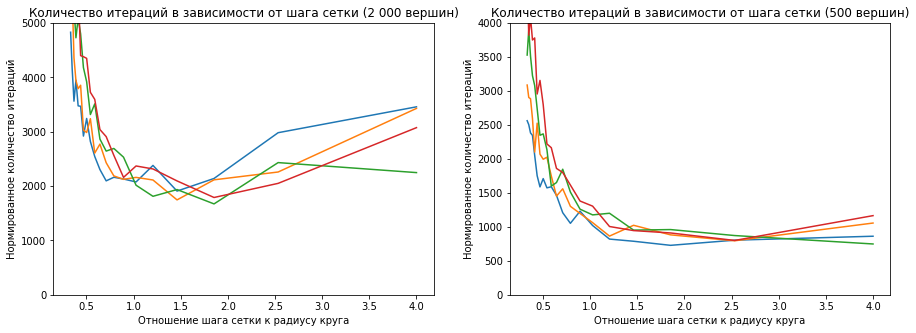
\includegraphics[width=\textwidth]{grid_step_2.png}
  \caption{Моделирование числа итераций локальных сил отталкивания для разных шагов сетки, значений $r_0$ и количеств вершин для размерности 2.}
  \label{fig:grid_step}
\end{figure}

Из-за неэффективой обработки условий в шейдерах WebGL, вычисление сил отталкивания будет проходить в два цикла: для {\bfseries локальных сил отталкивания} (для которых требуется обрабатывать вершины по одной) и {\bfseries глобальных} (когда считается силы между вершиной и клеткой).

При вычислении локальных сил, необходимо итерироваться по вершинам, входящих в некоторые клетки. Это добавляет еще один вложенный цикл, количество итераций которого равно максимальному числу вершин во всех клетках.

Таким образом, имеется три цикла, для которых необходимо иметь верхнюю оценку на число итераций (см. главу \ref{sec:webgl_data_analysis}). Оставшаяся часть этой главы будет посвящена объяснению выбора такой константы для последнего (вложенного) цикла, так как это влияет на реализацию алгоритма. Оценки для первых двух циклов будут даны в главе \ref{sec:repulsion_time} после главы с псевдокодом шейдера.

С учетом того, что число итераций вложенного цикла должно быть постоянным, имеет смысл брать лишь клетки одного уровня, так как в клетках разных уровней в разы отличается число входящих в них вершин.

Тогда задача состоит в том, чтобы найти шаг сетки, относительно круга радиуса $r_0$, для которых суммарное количество итераций наименьшее. Итерации происходят следующим образом. Выбираются те клетки, описанная окружность которых пересекаются с кругом радиуса $r_0$. Затем происходит обход вершин в выбранных клетках за время, равное произведению максимума числа вершин в во всех клетках сетки на число выбранных клеток.

При малом шаге сетки, у количества вершин в клетках будет большая дисперсия, а, следовательно, и максимум. При этом суммарная площадь выбранных клеток будет не сильно отличаться от площади круга. При большом шаге сетки, максимум количества вершин будет не значительно отличаться от среднего количества, но суммарная площадь выбранных клеток будет в разы больше площади круга.

Также следует заметить, что количество выбранных клеток зависит от положения центра круга относительно сетки и является случайной величиной. Но в реализации алгоритма число итераций должно равняться верхней оценке этого числа.

На рисунке \ref{fig:grid_step} показаны результаты моделирования количества итераций по схеме, описанной выше. Два графика показывают результаты при разном количестве вершин от $2\ 000$ и $500$. Разные линии в одном графике получены при разных значениях радиуса $r_0 = 1 / 20 \ldots 1 / 50$. Это соответствует разбросу параметров, например, от $7.5\%$ до $20\%$ точности при 8 уровнях. Наконец, каждая точка каждой линии была получена усреднением результатов на 10 случайных конфигурациях вершин. Вершины были равномерно распределены по квадрату. Так как при разных радиусах количество итераций значительно отличается, значения для каждой линии были домножены на величину, обратную радиусу, чтобы их можно было нанести на один график.

Как оказалось, оптимальный шаг сетки отличается при разной плотности вершин, но, в целом оптимальное значение находится в пределах $1.0 r_0 \ldots 2.0 r_0$. Для трех измерений шаг был около $2r_0\ldots 5r_0$.

В данной работе заначение шага сетки полагается равным $2r_0$. Помимо того, что оно находится в пределах оптимальных значений, для него количество клеток, которые пересекает круг, не превосходит 4, при этом эти четыре клетки содержатся в квадрате $2\times 2$, клетки которого можно получить при помощи столбцов 4H и 4L.

Так как клетки имеют стороны, равные обратным степеням двойки, шаг сетки выбирается как ближайшая сверху обратная степень двойки. Этот шаг хранится в константе \texttt{LOCAL\_GRID\_SIZE}.

Для того, чтобы иметь возможность итерироваться по клеткам квадрата $2\times 2$ в построенной выше сетки, необходимо потребовать, чтобы при построении дерева все клетки размера \texttt{LOCAL\_GRID\_SIZE} присутствовали, даже если в них нет вершин. Это увеличит размер текстуры для клеток, но ускорит процесс их прохода на GPU.

\section{Вычисление сил отталкивания при помощи иерархии клеток}

Структура для оптимизации вычисления сил отталкивания называется \texttt{grid} и имеет следующий поля:

\begin{itemize}
\item \texttt{grid.cells} --- RGBA текстура $4\times s$, где $s$ --- количество клеток.
\item \texttt{grid.vertices} --- дополнительная RGBA текстура, содержащая отсортированные номера вершин (см. описание в разделе \ref{sec:struct_texture}).
\item \texttt{grid.scale} --- вещественная константа, на которую домножаются 16-битные длины и координаты.
\end{itemize}

Далее приведен псевдокод шейдера вычисления сил отталкивания для размерности 2. Функции \texttt{low} и \texttt{high} приведены в листинге главы \ref{sec:attractions_implementation}.

\begin{verbatim}
calc_repulsions(vertex_no):
    float x = positions[vertex_no, 0]
    float y = positions[vertex_no, 1]
    float s = grid.scale
    int cell_no = 0
    float x_sum = 0, y_sum = 0, norm_sum = 0
    int top_left_cell_no = CELLS_COUNT

    for i = 1 .. GLOBAL_MAX_ITER:
        float side = high(grid.cells[cell_no, 0]) * s
        float dx = high(grid.cells[cell_no, 1]) * s - x
        float dy = low(grid.cells[cell_no, 1]) * s - y
        float sq_dist = dx ^ 2 + dy ^ 2
        float sq_accuracy = side ^ 2 / 2 / sq_dist;
        int next = low(grid.cells[cell_no, 0])
        int chebyshev = max(abs(dx), abs(dy))
        if grid_size == LOCAL_GRID_SIZE
           and chebyshev < side + LOCAL_GRID_SIZE:
             top_left_cell_no = min(top_left_cell_no, cell_no)
             cell_no = next
        elif sq_accuracy < SQ_MAX_ACCURACY:
            int count = low(grid.cells[cell_no, 2])
            float mul = calc_rep_mul(sq_dist) * mul
            norm_sum += mul
            x_sum += mul * dx, y_sum += mul * dy
            cell_no = next
        else:
            cell_no += 1
       if cell_no == 0 or cell_no >= CELLS_COUNT: break

    top_right_cell_no = high(grid.cells[top_left_cell_no, 4])
    bottom_left_cell_no = low(grid.cells[top_left_cell_no, 4])
    bottom_right_cell_no = high(grid.cells[bottom_left_cell_no, 4])

    x_add, y_add, norm_add = calc_local_forces(x, y, top_left_cell_no)
    x_sum += x_add, y_sum += y_add, norm_sum += norm_add
    x_add, y_add = calc_local_forces(x, y, top_right_cell_no)
    x_sum += x_add, y_sum += y_add, norm_sum += norm_add
    x_add, y_add = calc_local_forces(x, y, bottom_left_cell_no)
    x_sum += x_add, y_sum += y_add, norm_sum += norm_add
    x_add, y_add = calc_local_forces(x, y, bottom_right_cell_no)
    x_sum += x_add, y_sum += y_add, norm_sum += norm_add

    return x_sum, y_sum

calc_local_forces(x, y, cell_no)
    int vertex_min_idx = high(grid.cells[cell_no, 3])
    int vertex_max_idx = low(grid.cells[cell_no, 3])
    int cur_vertex_idx = vertex_min
    float x_sum = 0, y_sum = 0, norm_sum = 0
    for i = 1 .. MAX_GRID_VERTICES:
        if cur_vertex_idx > vertex_max_idx: break
        int vertex_no = low(grid.vertices[cur_vertex_idx])
        float dx = positions[vertex_no, 0] - x
        float dy = positions[vertex_no, 1] - y
        float sq_dist = dx ^ 2 + dy ^ 2
        float mul = calc_rep_mul(sq_dist)
        x_sum += dx * mul, y_sum += dy * mul, norm_sum += mul
        cur_vertex_idx += 1
    return x_sum, y_sum, norm_sum
\end{verbatim}

При вычислении локальных сил отталкивания расстояние возводится в квадрат, чтобы не брать квадратный корень.  Для определения пересечения квадратов используется расстояние Чебышева.

\begin{itemize}
\item Константа \texttt{SQ\_MAX\_ACCURACY} равна $\lambda^2$.
\item Константа \texttt{LOCAL\_GRID\_SIZE} равна шагу сетки, вычесленному в предыдущем разделе.
\item Константа \texttt{MAX\_GRID\_VERTICES} содержит максимальное количество вершин в клетке размера шага сетки. Предполагается, что во время выполнения обоих алгоритмов не будет клеток, в которых содержится значительно большее среднего число вершин.
\item Константа  \texttt{CELLS\_COUNT} содержит общее число клеток.
\item Переменная \texttt{top\_left\_cell\_no} хранит номер верхней левой клетки из тех четырех, которые используются для вычисления локальных сил отталкивания.
\item Переменная \texttt{norm\_sum} нужна для подсчета сумм норм в t-SNE, в Fruchterman Reingold её можно удалить.
\end{itemize}

Функция \texttt{calc\_rep\_mul} зависит от алгоритма:
\begin{verbatim}
calc_rep_mul_fruchterman_reingold(sq_dist):
    return -K_SQUARED / sqrt(sq_dist)

calc_rep_mul_tsne(sq_dist):
    return 1 / (1 + sq_dist)
\end{verbatim}

Константа \texttt{K\_SQUARED} равна квадрату \texttt{K} --- оптимальной длинны ребра в Fruchterman Reingold.

\section{Оценка времени вычисления сил отталкивания.}
\label{sec:repulsion_time}

Осталось найти оценку для константы \texttt{GLOBAL\_MAX\_ITER}, равной максимальному числу посещенных клеток при подсчете сил от одной вершины.

Сначала оценим количество вершин в дереве с $l$, $u$ листьями и не более $d$ потомками у каждого родителя. Пусть $l' = \lfloor\log_d u\rfloor$. Тогда первые $l'$ уровней содержат не более
$$d^0 + \cdots + d^{l'} = \frac{d^{l' + 1} - 1}{d - 1} < \frac{d u - 1}{d - 1} < \frac{d}{d - 1}$$
вершин. С другой стороны в каждом уровне число вершин не может превышать число всех листьев, поэтому число вершин в оставшихся $(l - l')$ уровнях не превосходит $u (l - l')$ и всего вершин не более
\begin{equation}
  \br{\frac{d}{d - 1} + l - \lfloor\log_d u\rfloor} u < \br{\frac{d}{d - 1} + l}u = C_1 u
  \label{eq:leafs_count}
\end{equation}

Рассмотрим дерево посещений, состоящее из всех клеток, запрошенных шейдером, приведенном в предыдущем разделе, при обработки одной вершины.

Оценим число листьев в дереве. Рассмотрим клетку со стороной $s$. Её <<радиус>> (то есть максимальное расстояние от вершины до центра квадрата) равен $r = s / \sqrt{2}$. Пусть клетка находятся на расстоянии $x$ от обрабатываемой шейдером вершины. Тогда для погрешности должно выполняться $r / x \le \lambda$. Если клетка является листом, то для её родителя, который в два раза больше, это условие должно нарушаться. Тогда $2r / x' > \lambda$, где $x'$ --- расстояние до центра родителя. Так как центр родителя совпадает с одним из углов дочерней клетки, $x' > x - r$. Получаем
$$\frac{r}{\lambda} \le x < x' + r < \br{\frac{2}{\lambda} + 1} r$$
Тогда все точки всех клеток (явяющихся листьями в дереве посещений) со стороной $s$ находятся в кольце с радиусом:
$$\br{\frac{1}{\lambda} - 1} r \ldots \br{\frac{2}{\lambda} + 2} r$$
Площадь этого кольца равна
$$\pi r^2 \br{(2 / \lambda + 2)^2 - (1/\lambda - 1)^2}$$
Чтобы получить оценку сверху на число квадратов в нем, необходимо разделить его площадь на $s^2 = 2r^2$, в результате получаем оценку
$$u < \frac{\pi}{2}\br{\frac{3}{\lambda^2} + \frac{10}{\lambda} + 3} (l - l_0),$$
где $l_0 = \log_2(1 / \lambda) - 1$ --- верхняя оценка на слой клетки, являющейся листовой (см. главу \ref{sec:cells_implementation}).

Подставляя оценку на $u$ в формулу \ref{eq:leafs_count}, получаем верхнюю оценку на число глобальных итераций.

\section{Результаты испытаний}

\begin{table}[t]
  \centering
  \begin{tabular}{|l l l l l|}
    \hline
     &  & время & $\sigma$ & итераций \\ \hline
    \texttt{attractions} & \texttt{JS} & 0.706 & $\pm 0.023$ & 10 \\ \cline{2-5}
             & \texttt{JS + WebGL} & 0.00111 & $\pm 0.000023$ & 1000 \\\hline
    \texttt{repulsions} & \texttt{C} & 0.671 & $\pm 0.05$ & 10 \\ \cline{2-5}
     & \texttt{asm.js} & 0.514 & $\pm 0.011$ & 10 \\\cline{2-5}
     & \texttt{JS} & 0.504 & $\pm 0.009$ & 10 \\\cline{2-5}
             & \texttt{JS + WebGL} & 0.0247 & $\pm 0.00013$ & 1000 \\\hline
  \end{tabular}
  \caption{Результаты испытаний}
  \label{tab:myfirsttable}
\end{table}

Испытания проводились отдельно для сил отталкивания и притяжения. Измерялось время одной итерации в секундах. Код делился подготовительную и основную часть. В подготовительную часть включалась генерация начальных значений и компиляция. Для реализаций на WebGL время на пересылку от CPU к GPU и обратно включалось в основную часть. Перед началом измерений делалось $30\%$ итераций для <<разогрева>>.

Испытания проводились на 64-битном двухъядерном процессоре Intel Core i3-2330M (2.20 GHz) в браузере Chromium 66. В качестве GPU использовался интегрированный графический процессор Intel HD Graphics 3000 с 12 ядрами.

Для сил отталкивания сравнивались простые реализации (имеющие квадратичную сложность) на графе из 4096 вершин. Начальные положения точек генерировались при помощи псевдо-случайного алгоритма с одинаковым начальным значением.

Неожиданный результат был получен при сравнении реализаций на \texttt{C}, \texttt{asm.js} и \texttt{JS}. Код на \texttt{C} был скомпилирован с флагами \texttt{-lm -Ofast}, тем не менее, время его выполнения оказалось на $30\%$ медленнее, чем аналогичного кода на \texttt{JS}, при том, что оптимизированная версия на \texttt{asm.js} показала такой же результат, как и обычная реализация на \texttt{JS}. В реализации на WebGL пересылка от CPU к GPU и обратно проводилась один раз на 10 итераций.

Для сил притяжения использовался граф из 4096 вершин и $4096 \times 1000$ ребер. Каждая вершина имела по 2000 исходящих ребер, константа для схемы (s) равнялась 1000, то есть на каждую вершину приходилось две строки по 1000 ребер. Время вычисления всех сил на GPU (включая пересылку) было сравнимо со временем обхода всех вершин в цикле на JS с выполнением одной простой операции, например, суммы.

\chapter{Подробности реализации веб-приложения}

\section{Разделение приложения на компоненты}

В JavaScript существует множество фреймворков для создания компонентов, в данном проекте используется React. Изначально он создавался как эффективное средство для манипуляции DOM, но, как оказалось, может использоваться и для работы с сущностями, не имеющих DOM-представления. Например, главный файл компоненты-<<проигрывателя>>, упрощенно, выглядит так (пропущенный код заменен на многоточия):
\begin{verbatim}
  <SimpleDownloader downloads={...}>
    {({ baseFile, patchFile }) => {
      ... return (
        <FullScreen>
          {({ width, height }) => (
            <Viewport3d initialTarget={target} ...>
              {({target, viewport, setTarget, setViewport, ...}) => {
                ... return (
                  <WebGLCanvas
                    data={{viewport: [width / 2, height / 2, height],
\end{verbatim}
Приведенные выше компоненты имеют следующие функции:
\begin{itemize}
\item \texttt{SimpleDownloader} --- ожидает загрузки переданных ему объектов. Может одновременно делать несколько загрузок. При загрузке показывает процент загруженных данных, если сервер предоставляет такую информацию. После загрузки передает файлы в виде JSON-объектов дочернему компоненту.
\item \texttt{FullScreen} --- измеряет размер экрана и передает его размеры дочернему компоненту. В случае изменения размеров окна информирует об этом дочерние компоненты через механизм обновления React.
\item \texttt{Viewport3d} --- контролирует камеру в трехмерном пространстве. Реагирует на события мыши в дочерних компонентах (через вызов callback) и сообщает дочерним элементам обновленную матрицу преобразования.
\item \texttt{WebGLCanvas} --- основной компонент, отвечающий за рендер WebGL сцены. Это единственный компонент здесь, имеющий DOM-представление.
\end{itemize}

\section{Описание формата хранения интерактивных визуализаций}

\label{sec:format}

Идея состоит в том, чтобы максимально точно повторить семантику работы WebGL. Это делает формат пригодным только для выполнения в браузере, но в то же время делает его крайне эффективным.

Так как в этом формате нет возможности вставки кода на JavaScript, единственный способ добавить интерактивность состоит в том, чтобы делать все анимации и вычисления в шейдерах. Благодаря этому все данные передаются с CPU на GPU только один раз, после этого происходит только изменение uniform-переменных, которые занимают по несколько байт и передаются очень быстро.

Как оказалось, практически все анимации можно успешно выполнить в шейдерах. Основная uniform-переменная для этого --- это время \texttt{t}. Но, в случае необходимости, можно добавить и другие переменные, которые могут контролироваться через интерфейс. \texttt{camera} --- другая важная переменная, содержащая матрицу камеры, которой можно управлять мышкой через интерфейс пользователя.

Несмотря на использование WebGL, в этом формате можно также успешно реализовывать и плоские визуализации. Достаточно зафиксировать направление камеры и заменить вращение на перемещение.

В этом формате также решена проблема интерактивности --- при наведении курсора на текст в интерфейс передаётся информация о выбранном объекте. Для этого используется дополнительная невидимая текстура, каждый RGBA-пиксель которой хранит номер текущего объекта. Это позволяет отличать 65535 объектов, что достаточно для большинства приложений.

Для рендера видео была добавлена поддержка пост-эффектов, которые применяются к результату работы шейдера. Так как WebGL нет возможности считать буфер глубины (без использования расширений, которые поддерживаются не всеми устройствами), информация о расстоянии до камеры сохраняется в alpha-канале. Это позволяет добавлять пост-эффекты, зависящие от расстояния до камеры, например, lens blur.

Основным форматом хранения был выбран JSON. Единственная его проблема состоит в том, что массивы вещественных чисел требуют больше символов для записи, чем в бинарном формате. Для решения этой проблемы в будущем может быть добавлена возможность прикреплять файл с двоичными данными и в JSON вместо массива чисел передавать адреса начала и конца массива в двоичном файле, а также информацию о его типе.

Чтобы избежать проблемы с копированием данных в разных модификациях одной визуализации, добавляется новый тип файла: <<патч>>. Он ссылается на <<родительский>> файл и содержит только те поля JSON, которые были изменены. Тогда перед воспроизведением <<патч>>-файл объединяется с <<родительским>> файлом при помощи операции, которая в функциональных языках называется \texttt{MergeDeepRight}.

Большинство полей этого формата можно анимировать. Для этого достаточно передать массив значений вместо одного значения или массив кратно большей длины там, где требуется массив. Тогда в кадре с соответствующим номером будет использоваться соответствующее значение. Так можно отображать некоторые слои лишь на некоторых кадрах или рисовать один и тот же слой несколько раз в одном кадре. Также можно выбирать подмассив элементов для рисования в вызове gl.DrawArrays.

При анимировании параметров слоя номер кадра соотносится с массивом frames данного слоя. Это позволяет отображать один слой несколько раз с разными параметрами во время рисования одного кадра.

Наконец, при необходимости изменить какие-либо подмножества буффера или текстуры, во время воспроизведения визуализации можно вызвать метод объекта, ответственного за управление Canvas. Это используется, например, при динамическом рисовании графа при помощи алгоритма Fruchterman Reingold.

Также, например, для изменения ширины и высоты визуализации при изменении размеров окна можно добавлять еще один <<патч>> и передавать его объекту, ответственного за управление Canvas. Совпадающие поля будут перезаписаны на новые значения.

Далее идет описание основных полей этого JSON:

\begin{itemize}
\item \texttt{width}, \texttt{height} --- ширина и высота результата визуализации в пикселях.
\item \texttt{parent} --- название родительского файла для <<патч>>-файлов.
\item \texttt{start}, \texttt{step}, \texttt{stop} --- информация об интервале воспроизведения. Это полезно при работе над длинной анимацией, чтобы при отладке сразу перейти к интересующему отрывку. Параметр step нужен, если время рендера сцены долгое и необходимо сделать быстрый предпросмотр отдельных кадров.
\item \texttt{background} --- цвет сцены в местах, где нет объектов. Передается в функцию gl.clearColor.
\item \texttt{programs} --- словарь, содержащий все шейдеры, используемые в визуализации. Ключами словаря являются идентификаторы програм.
\item \texttt{programs[programId].uniforms} --- словарь, содержащий типы uniform-переменных шейдера. Теоретически, эту информацию можно получить, распарсив шейдер, но в этой версии формата её необходимо передавать явно.
\item \texttt{programs[programId].textures} --- словарь, содержащий номера активных текстур, к которым необходимо прикреплять переменные. Эта информация позволяет эффективнее переключать текстуры.
\item \texttt{programs[programId].attributes} --- словарь, содержащий информацию о типах аттрибутов. Аналогично с uniforms, эту информацию можно было бы извлекать из кода шейдера.
\item \texttt{programs[programId].vertex} --- код вершинного шейдера.
\item \texttt{programs[programId].fragment} --- код фрагментного шейдера.
\item \texttt{programs[programId].mode} --- режим отображения объектов. Может принимать значения: POINTS, TRIANGLES, LINES и т.д.
\item \texttt{buffers} --- словарь, содержащий информацию о буфферах (которые присваиваются аттрибутам) в визуализации.
\item \texttt{buffers[bufferId].type} --- тип данных буффера. Может принимать значения Uint8Array, Float32Array и т.д.
\item \texttt{buffers[bufferId].data} --- собственнно, данные буффера.
\item \texttt{buffers[bufferId].is\_index} --- является ли буффер индексным (то есть вызывается ли gl.DrawElements или gl.DrawArrays).
\item \texttt{buffers[bufferId].item\_size} --- размер вектора, передаваемого одному объекту.
\item \texttt{textures} --- словарь, содержащий информацию о текстурах.
\item \texttt{textures[textureId].filter} --- фильтр для изображения. Может принимать значения NEAREST, LINEAR и т.д.
\item \texttt{textures[textureId].url} --- url изображения для текстуры.
\item \texttt{layers} --- словарь, содержащий слои. В слоях содержится информация об объектах, рисуемых на сцене.
\item \texttt{layers[layerId].program} --- идентификатор шейдера, используемой в данном слое.
\item \texttt{layers[layerId].frames} --- массив, содержащий перенумерацию кадров для анимирования других параметров данного слоя. Это позволяет отображать слой в некоторых кадрах или отображать его несколько раз с разными параметрами в пределах одного кадра. 
\item \texttt{layers[layerId].uniforms} --- значения uniform-переменных для данного слоя. Эти переменные должны анимироваться в первую очередь. 
\item \texttt{layers[layerId].attributes} --- словарь, сопоставляющий аттрибутам идентификаторы буфферов.
\item \texttt{layers[layerId].textures} --- словарь, сопоставляющий uniform-переменным номера активных текстур.
\item \texttt{layers[layerId].draw} --- параметры рисования слоя.
\item \texttt{layers[layerId].draw.first} --- индекс первого элемента для рисования.
\item \texttt{layers[layerId].draw.count} --- количество элементов для рисования.
\item \texttt{camera} --- информация о камере.
\item \texttt{camera.near} --- расстояние до ближайшего объекта, отображаемого камерой.
\item \texttt{camera.far} --- расстояние до самого дальнего объекта, отображаемого камерой.
\item \texttt{camera.fov} --- вертикальный угол поля зрения камеры в градусах.
\item \texttt{camera.target} --- трехмерные координаты точки, на которую направлена камера
\item \texttt{camera.polar} --- эйлеровы углы направления камеры.
\item \texttt{postprocessing} --- информация о пост-эффектах. Имеет тех же потомков, что и каждый отдельный слой. Помимо этого, имеет три дополнительных параметра.
\item \texttt{postprocessing.post\_iters} --- количество внешних итераций пост-шейдера. 
\item \texttt{postprocessing.blend\_iters} --- количество внутренних итераций пост-шейдера.
\item \texttt{postprocessing.motion\_blur} --- коэффициент размытия motion blur.
\end{itemize}

\section{Отображение большого количества текста в WebGL}

Одним из недостатков WebGL и OpenGL является отсуствие простой возможности добавить текстовую подпись на сцену. Есть следующие подходы к решению этой проблемы:

\begin{itemize}
\item Рисование всех надписей в Canvas2D и передача их в виде одной или нескольких текстур.
\item Превращение каждой буквы в набор треугольников рисование ихсредствами WebGL.
\item Создание текстуры для каждой буквы и составление слов из отдельных букв.
\end{itemize}

В визуализациях, создаваемых в системе, может быть порядка $15\ 000$ надписей, что делает слишком неэффективным по использованию памяти и времени применение первого и второго способа. Поэтому был выбран третий способ.

Другая проблема заключалась в том, что иногда надписи оказывались прямо перед камерой и были заметны контуры пикселей. Такую проблему обычно решают при помощи signed distance field. Но на практике оказалась рабочей более простая техника: достаточно применить к текстуре буквы сначала билинейную интерполяцию (которая включается стандартной командой WebGL), затем в шейдере сделать threshold с порогом 0.5. Преимущество этого метода состоит также в том, что такую текстуру можно легко сгенерировать для любого шрифта без использования специальных утилит.

Последняя оптимизация заключалась в использовании точечного шейдера (gl.POINTS) для рисования букв. Это в разы улучшило скорость рисования и потребление памяти для буфферов, но создавало ограничения на максимальную высоту букв в 255 пикселей. Поэтому пришлось отказаться от показа надписей, которые слишком близко к камере.

Для генерации текстуры шрифтов использовалась библиотека двумерного рисования Cairo, имеющая API для python. Для улучшения читаемости текста, в другом канале текстуры содержалась обводка букв. Данные о позициях и координатах букв хранились в отдельном json-файле.

\section{Проблема отображения полупрозрачных объектов}

Одной из проблем, не имеющих универсального решения в OpenGL и WebGL является отображение полупрозрачных объектов.

При неправильном порядке рисования полупрозрачные объекты будут выглядеть неестественно. Первое решение состоит в том, чтобы перед рисованием объекты отсортировать. У этого решения есть следующие проблемы:

\begin{itemize}
\item Сортировка требует много времени CPU.
\item Недостаточно сортировать по расстоянию до камеры: довольно часто возникают ситуации, когда при такой сортировке возникают видимые дефекты.
\item Если объекты пересекаются, сортировка не может дать правильный результат.
\item Стандартный алгоритм рисования объектов в WebGL не гарантирует порядок рисования объектов. Для рисования по порядку необходимо запускать метод drawArrays множество раз, что несколько раз медленнее.
\end{itemize}

Решение, предлагаемое в данной работе, следующее: при рисовании объекта прозрачности $\alpha$ применять к нему такой шейдер, который рисует каждый пиксель объекта независимо с вероятностью $\alpha$. Это делается при помощи специальной команды discard в языке шейдеров, которая делает текущий пиксель полностью прозрачным. Тогда при усреднени большого числа итераций таких шейдеров среднее значение пикселя будет в точности равно требуемому.

С учетом необходимости производить рисование одного и того же кадра множество раз, полупрозрачноть может использоваться только при создании видео.

\section{Рендер видео и пост-эффекты.}

При разработке приложения было важно сделать возможность производить рендер видео с пост-эффектами при помощи того же движка, что и для интерактивных визуализаций. Это ускоряло процесс прототипирования и увеличивало переиспользование кода.

Оказалось, что схема мультисэмплинга, используемая для получения полупрозрачности, позволяет создавать другие пост-эффекты, полезные при создании видео:

\begin{itemize}
\item {\bfseries Antialiasing.} Достаточно в вершинных шейдерах случано сдвигать координаты всех вершин на $\pm 0.5$ пикселя.
\item {\bfseries Motion blur.} Во время интерполяции анимированных значений (в JSON-файле формата, описанного в главе \ref{sec:format}) достаточно добавить случайное число $\pm 0.5$ кадра.
\end{itemize}

Для сохранения видео на той же машине запускался простой веб-сервер на Python Tornado, который получал POST-запросы с base64-закодированным png-изображением для каждого кадра и сохранял их под последовательными номерами. Затем при помощи консольной утилиты ffmpeg кадры конвертировались в видео.

Также возможен следующий варант совмещения пост-эффектов с интерактивным режимом. Если в кадре ничего не меняется, происходит <<накопление>> одиночных рендеров сцены в экранный буффер. Как только положение камеры меняется, экранный буффер сбрасывается. Таким образом, при изменении сцены показывается предпросмотр сцены с низким качеством (но быстрым откликом), и по мере того, как камера остается неподвижной, качество отображения постепенно улучшается. 

\section{Мультисэмплинг на WebGL 1}

Для мультисэмплинга можно было использовать команду renderbufferStorageMultisample из WebGL 2 API (которая поддерживается не всеми устройствами), либо производить его вручную методами WebGL 1.

В WebGL 1 мультисэмплинг осуществлялся следующим образом. Обозначим $r^{(i)}$ --- значение нового кадра на итерации $i$, а $f^{(i)}$ --- значение буффера, <<накапливающего>> среднее значение. Тогда простая схема проводилась по формуле:
$$f^{(i)} = f^{(i-1)} \br{1 - \frac{1}{i}} + r^{(i)} \frac{1}{i},$$
то есть
$$f^{(1)} = r^{(1)},\quad f^{(i)} = \frac{r^{(1)} + \cdots + r^{(i)}}{i}.$$
Проблема заключалась в том, что и буффер $r$ и буффер $f$ имели по 256 градаций каждого цвета и усредненное значение имело меньше градаций оттенков из-за накапливающихся ошибок округления.

Решение заключалось в создании дополнительного буффера $h$ по правилу
$$h^{(ik)} = h^{((i - 1)k)} \br{1 - \frac{1}{i}} + f^{(ik)}\frac{1}{i},$$
при этом каждые $k$ итераций буффер $f$ <<сбрасывался>>.
Параметр $k$ можно было выбирать при помощи поля \texttt{postprocessing.blend\_iters}.

\section{Lens blur.}

Самым сложным пост-эффектом оказался lens blur. Он был реализован в предположении, что <<диафрагма>> объектива имеет круглую форму, а объекты, находящиеся ближе, чем фокусное расстояние, не теряли четкости.

Фрагмент кода шейдера приведен ниже:
\begin{verbatim}
vec3 sum = cur_tex.xyz;
float count = 1.0;
float coeff = max(0.0, 1.0 - beta * cur_tex.a)
float rad = pow(rand(), 0.5) * alpha * coeff;
float min_a = (1.0 - rad / alpha) / beta;
for (int i=0; i<ITERS; i++) {
    float a = rand().x * PI * 2;
    vec2 delta = rad * vec2(cos(a), sin(a));
    vec4 tex = texture2D(render, gl_FragCoord.xy + delta);
    if (tex.a > min_a) continue;
    sum += tex.xyz;
    count += 1.0;
}
return sum / count;
\end{verbatim}
В alpha-канале хранится вещественное число, обратно пропорциональное расстоянию до камеры. Идея состоит в подсчете среднего по случайной выборке соседних пикселей, при этом каждый пиксель берется с вероятностью, пропорциональной степени его размытия. Для ускорения вычислений, расстояние от текущего пикселя, на котором берется случайный пиксель, фиксируется для всех итераций. Так как шейдер запускается множество раз, распределение векторов \texttt{delta} будет образовывать круг необходимого радиуса.
\begin{itemize}
\item \texttt{alpha} --- значение диафрагмы,
\item \texttt{beta} --- фокусное расстояние,
\item \texttt{cur\_tex} --- значение обрабатываемого пикселя,
\item \texttt{sum} --- накапливаемая сумма значений пикселей,
\item \texttt{count} --- количество накопленных пикселей,
\item \texttt{coeff} --- отношение радиуса размытия для текущего пикселя по сравнению с максимальным,
\item \texttt{rand()} --- функция генерации случайного числа из отрезка $[0, 1]$,
\item \texttt{rad} --- случайная точка в радиусе размытия текущего пикселя,
\item \texttt{min\_a} --- минимальное значение alpha-канала для того, чтобы пиксель был добавлен к накопленному значению,
\item \texttt{ITERS} --- количество проверок ближайших пикселей,
\item \texttt{a} --- случайный угол,
\item \texttt{delta} --- случайный вектор длины \texttt{rad},
\item \texttt{tex} --- значние случайного пикселя, в направлении \texttt{delta} от текущего пикселя.
\end{itemize}

\begin{thebibliography}{99}

\bibitem{communities} Blondel, Vincent D., et al. "Fast unfolding of communities in large networks." Journal of statistical mechanics: theory and experiment 2008.10 (2008): P10008.

\bibitem{acc_tsne} Van Der Maaten, Laurens. "Accelerating t-SNE using tree-based algorithms." Journal of machine learning research 15.1 (2014): 3221-3245.

\bibitem{barnes_hut} Barnes, J. Fritz and Piet Hut. “A hierarchical O(N log N) force-calculation algorithm.” Nature 324 (1986): 446-449.

\bibitem{v2w_length} Schakel, Adriaan MJ, and Benjamin J. Wilson. "Measuring word significance using distributed representations of words." arXiv preprint arXiv:1508.02297 (2015).

\bibitem{tsne} Maaten, Laurens van der, and Geoffrey Hinton. "Visualizing data using t-SNE." Journal of machine learning research 9.Nov (2008): 2579-2605.

\bibitem{weighted_layout} Vrajitoru, Dana, and Jason DeBoni. "Consistent graph layout for weighted graphs." Computer Systems and Applications, 2005. The 3rd ACS/IEEE International Conference on. IEEE, 2005.

\bibitem{graph_2d_survey} Gibson, Helen, Joe Faith, and Paul Vickers. "A survey of two-dimensional graph layout techniques for information visualisation." Information visualization 12.3-4 (2013): 324-357.

\bibitem{graph_nlp_survey} Nastase, Vivi, Rada Mihalcea, and Dragomir R. Radev. "A survey of graphs in natural language processing." Natural Language Engineering 21.5 (2015): 665-698.

\bibitem{graph_navigation} Herman, Ivan, Guy Melançon, and M. Scott Marshall. "Graph visualization and navigation in information visualization: A survey." IEEE Transactions on visualization and computer graphics 6.1 (2000): 24-43.

\bibitem{interactive_tpp} Gibson, Helen, and Paul Vickers. "graphTPP: A multivariate based method for interactive graph layout and analysis." arXiv preprint arXiv:1712.05644 (2017).

\bibitem{3d_vis_info} Young, Peter. "Three dimensional information visualisation." (1996).

\bibitem{interactive_relations} Dörk, Marian, Sheelagh Carpendale, and Carey Williamson. "Visualizing explicit and implicit relations of complex information spaces." Information Visualization 11.1 (2012): 5-21.

\bibitem{interactive_large_graph} Wills, Graham J. "NicheWorks—interactive visualization of very large graphs." International Symposium on Graph Drawing. Springer, Berlin, Heidelberg, 1997.

\bibitem{forceatlas2} Jacomy, Mathieu, et al. "ForceAtlas2, a continuous graph layout algorithm for handy network visualization designed for the Gephi software." PloS one 9.6 (2014): e98679.

\bibitem{interactive_graph_3d_fast} Bruß, Ingo, and Arne Frick. "Fast interactive 3-D graph visualization." International Symposium on Graph Drawing. Springer, Berlin, Heidelberg, 1995.

\bibitem{fr} Fruchterman, Thomas MJ, and Edward M. Reingold. "Graph drawing by force‐directed placement." Software: Practice and experience 21.11 (1991): 1129-1164.

\bibitem{graph_3d_clustered} Ho, Joshua, and Seok-Hee Hong. "Drawing clustered graphs in three dimensions." International Symposium on Graph Drawing. Springer, Berlin, Heidelberg, 2005.

\bibitem{interactive_3d_graph} Ahmed, Adel, et al. "Geomi: Geometry for maximum insight." International Symposium on Graph Drawing. Springer, Berlin, Heidelberg, 2005.

\bibitem{classic_3d_trees} Robertson, George G., Jock D. Mackinlay, and Stuart K. Card. "Cone trees: animated 3D visualizations of hierarchical information." Proceedings of the SIGCHI conference on Human factors in computing systems. ACM, 1991.

\bibitem{book_graph_drawing} Tamassia, Roberto, Giuseppe Di Battista, and Carlo Batini. "Automatic graph drawing and readability of diagrams." IEEE Transactions on Systems, Man, and Cybernetics 18.1 (1988): 61-79.

\bibitem{interactive_document_exploration} Görg, Carsten, et al. "Combining computational analyses and interactive visualization for document exploration and sensemaking in jigsaw." IEEE Transactions on Visualization and Computer Graphics 19.10 (2013): 1646-1663.

\bibitem{cooc_graph} Ohsawa, Yukio, Nels E. Benson, and Masahiko Yachida. "KeyGraph: Automatic indexing by co-occurrence graph based on building construction metaphor." Research and Technology Advances in Digital Libraries, 1998. ADL 98. Proceedings. IEEE International Forum on. IEEE, 1998.

\bibitem{evolving_graph} Erten, Cesim, et al. "GraphAEL: Graph animations with evolving layouts." International Symposium on Graph Drawing. Springer, Berlin, Heidelberg, 2003.

\bibitem{book_force} Kobourov, Stephen G. "Spring embedders and force directed graph drawing algorithms." arXiv preprint arXiv:1201.3011 (2012).

\bibitem{graph_spring} Kobourov, Stephen G. "Spring embedders and force directed graph drawing algorithms." arXiv preprint arXiv:1201.3011 (2012).

\bibitem{graph_interactive} Tominski, Christian, James Abello, and Heidrun Schumann. "CGV—An interactive graph visualization system." Computers \& Graphics 33.6 (2009): 660-678.

\bibitem{in_situ} Hadlak, Steffen, Hans-Jorg Schulz, and Heidrun Schumann. "In situ exploration of large dynamic networks." IEEE Transactions on Visualization and Computer Graphics 17.12 (2011): 2334-2343.

\bibitem{scalable_web} retarsson, Brynjar, et al. "WiGis: A framework for scalable web-based interactive graph visualizations." International Symposium on Graph Drawing. Springer, Berlin, Heidelberg, 2009.

\bibitem{bio_graph} Adai, Alex T., et al. "LGL: creating a map of protein function with an algorithm for visualizing very large biological networks." Journal of molecular biology 340.1 (2004): 179-190.

\bibitem{25d_interactive_graph} Itoh, Masahiko, Masashi Toyoda, and Masaru Kitsuregawa. "An interactive visualization framework for time-series of web graphs in a 3D environment." Information Visualisation (IV), 2010 14th International Conference. IEEE, 2010.

\bibitem{large_document} Chen, Yanhua, et al. "Exemplar-based visualization of large document corpus (infovis2009-1115)." IEEE Transactions on Visualization and Computer Graphics 15.6 (2009).

\bibitem{phrase_graph} Van Ham, Frank, Martin Wattenberg, and Fernanda B. Viégas. "Mapping text with phrase nets." IEEE transactions on visualization and computer graphics 15.6 (2009).

\bibitem{meme_tracking} Leskovec, Jure, Lars Backstrom, and Jon Kleinberg. "Meme-tracking and the dynamics of the news cycle." Proceedings of the 15th ACM SIGKDD international conference on Knowledge discovery and data mining. ACM, 2009.

\bibitem{word_tree} Wattenberg, Martin, and Fernanda B. Viégas. "The word tree, an interactive visual concordance." IEEE transactions on visualization and computer graphics 14.6 (2008).

\bibitem{classic_ecologies} Chi, Ed H., et al. "Visualizing the evolution of web ecologies." Proceedings of the SIGCHI conference on Human factors in computing systems. ACM Press/Addison-Wesley Publishing Co., 1998.

\bibitem{interactive_layered_graph} Nakazono, Nagayoshi, Kazuo Misue, and Jiro Tanaka. "NeL 2: network drawing tool for handling layered structured network diagram." Proceedings of the 2006 Asia-Pacific Symposium on Information Visualisation-Volume 60. Australian Computer Society, Inc., 2006.

\bibitem{25d_vislink} Collins, Christopher, and Sheelagh Carpendale. "VisLink: Revealing relationships amongst visualizations." IEEE Transactions on Visualization and Computer Graphics 13.6 (2007): 1192-1199.

\bibitem{25d_simultaneous} Erten, Cesim, et al. "Simultaneous graph drawing: Layout algorithms and visualization schemes." International Symposium on Graph Drawing. Springer, Berlin, Heidelberg, 2003.

\bibitem{hyperbolic} Lamping, John, Ramana Rao, and Peter Pirolli. "A focus+ context technique based on hyperbolic geometry for visualizing large hierarchies." Proceedings of the SIGCHI conference on Human factors in computing systems. ACM Press/Addison-Wesley Publishing Co., 1995.

\bibitem{visual_data_mining} Kreuseler, Matthias, and Heidrun Schumann. "A flexible approach for visual data mining." IEEE Transactions on Visualization and Computer Graphics 8.1 (2002): 39-51.

\bibitem{interactive_coordinated_views} Roberts, Jonathan C. "State of the art: Coordinated \& multiple views in exploratory visualization." Coordinated and Multiple Views in Exploratory Visualization, 2007. CMV'07. Fifth International Conference on. IEEE, 2007.

\bibitem{25d_bloggers} Itoh, Masahiko, et al. "Analysis and visualization of temporal changes in bloggers' activities and interests." Visualization Symposium (PacificVis), 2012 IEEE Pacific. IEEE, 2012.

\bibitem{large_graph_survey} Jarukasemratana, Sorn, and Tsuyoshi Murata. "Recent large graph visualization tools: a review." Information and Media Technologies 8.4 (2013): 944-960.

\end{thebibliography}



\chapter{Приложение. Примеры визуализаций}

\begin{figure}[h]
  \centering
  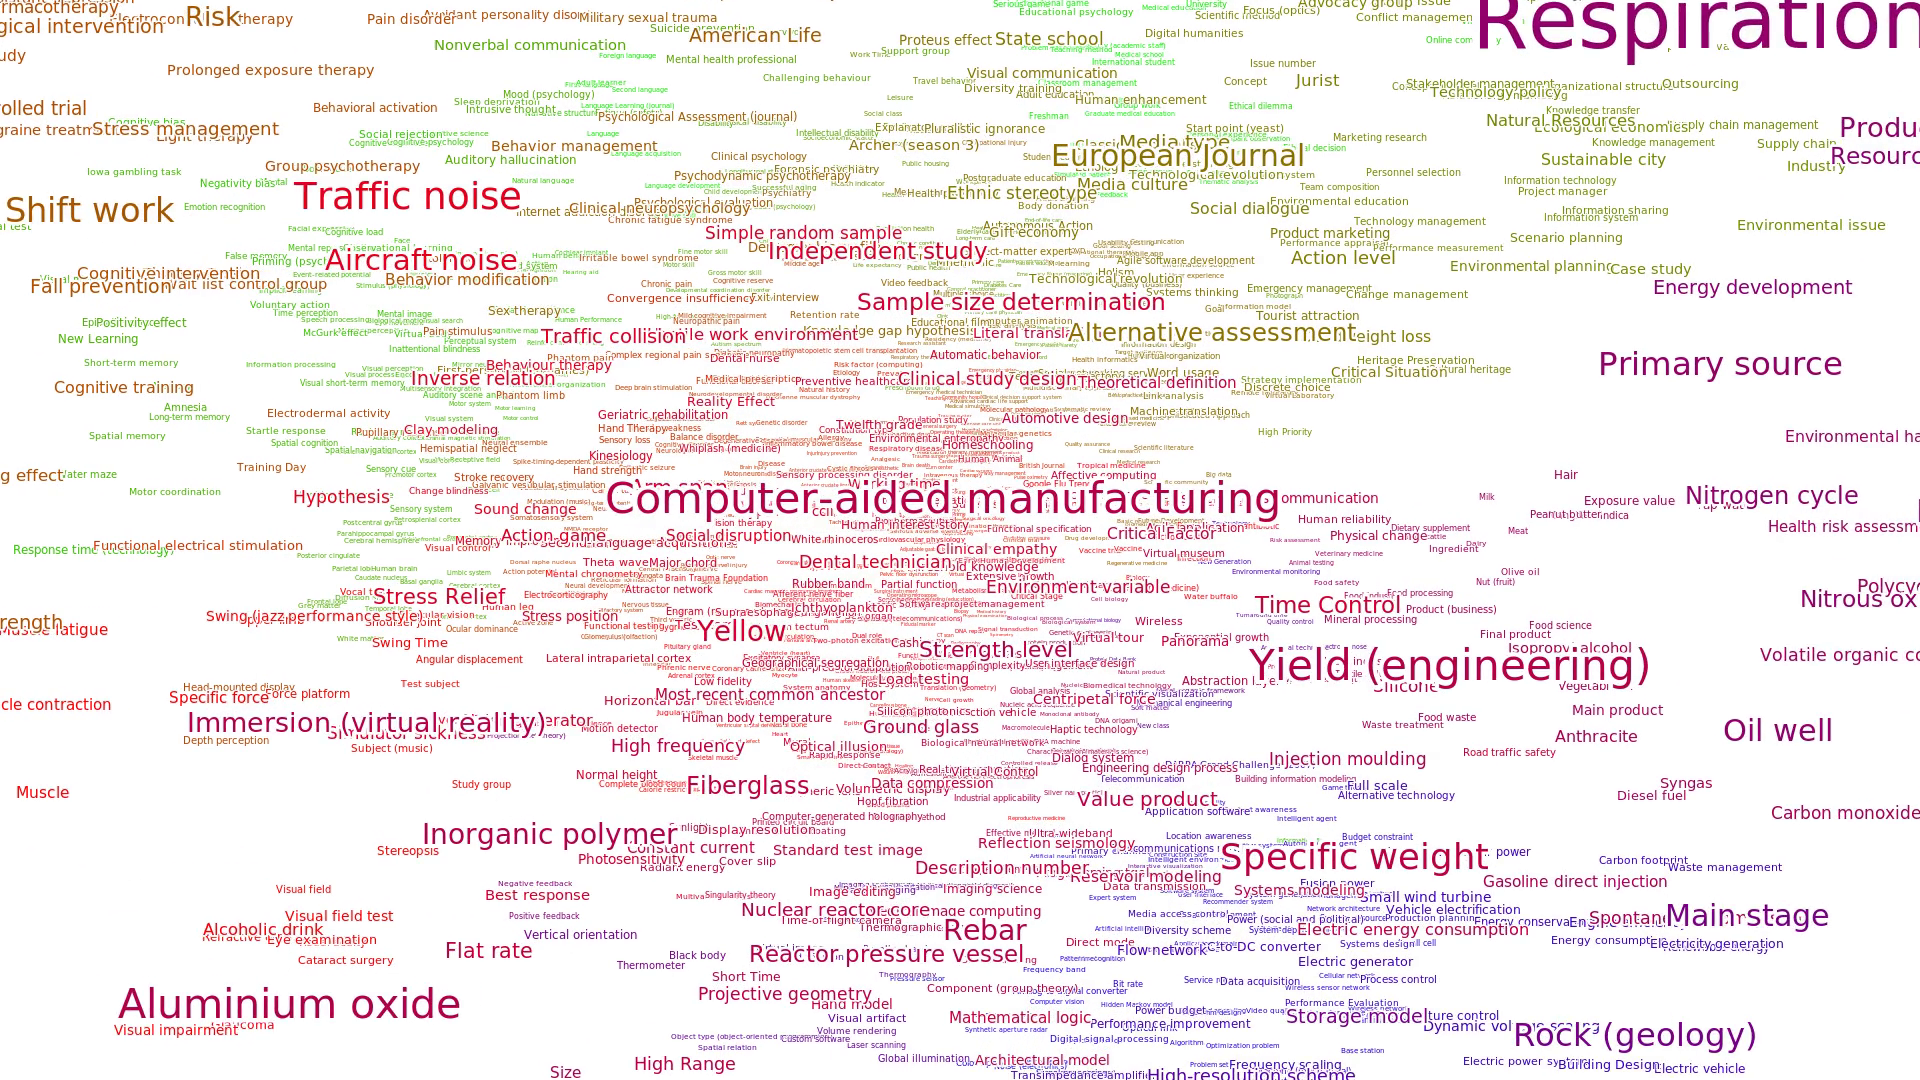
\includegraphics[width=\textwidth]{shots/cloud.png}
  \caption{Облако слов, полученное применением трехмерного t-SNE к word2vec.}
\end{figure}

\begin{figure}[h]
  \centering
  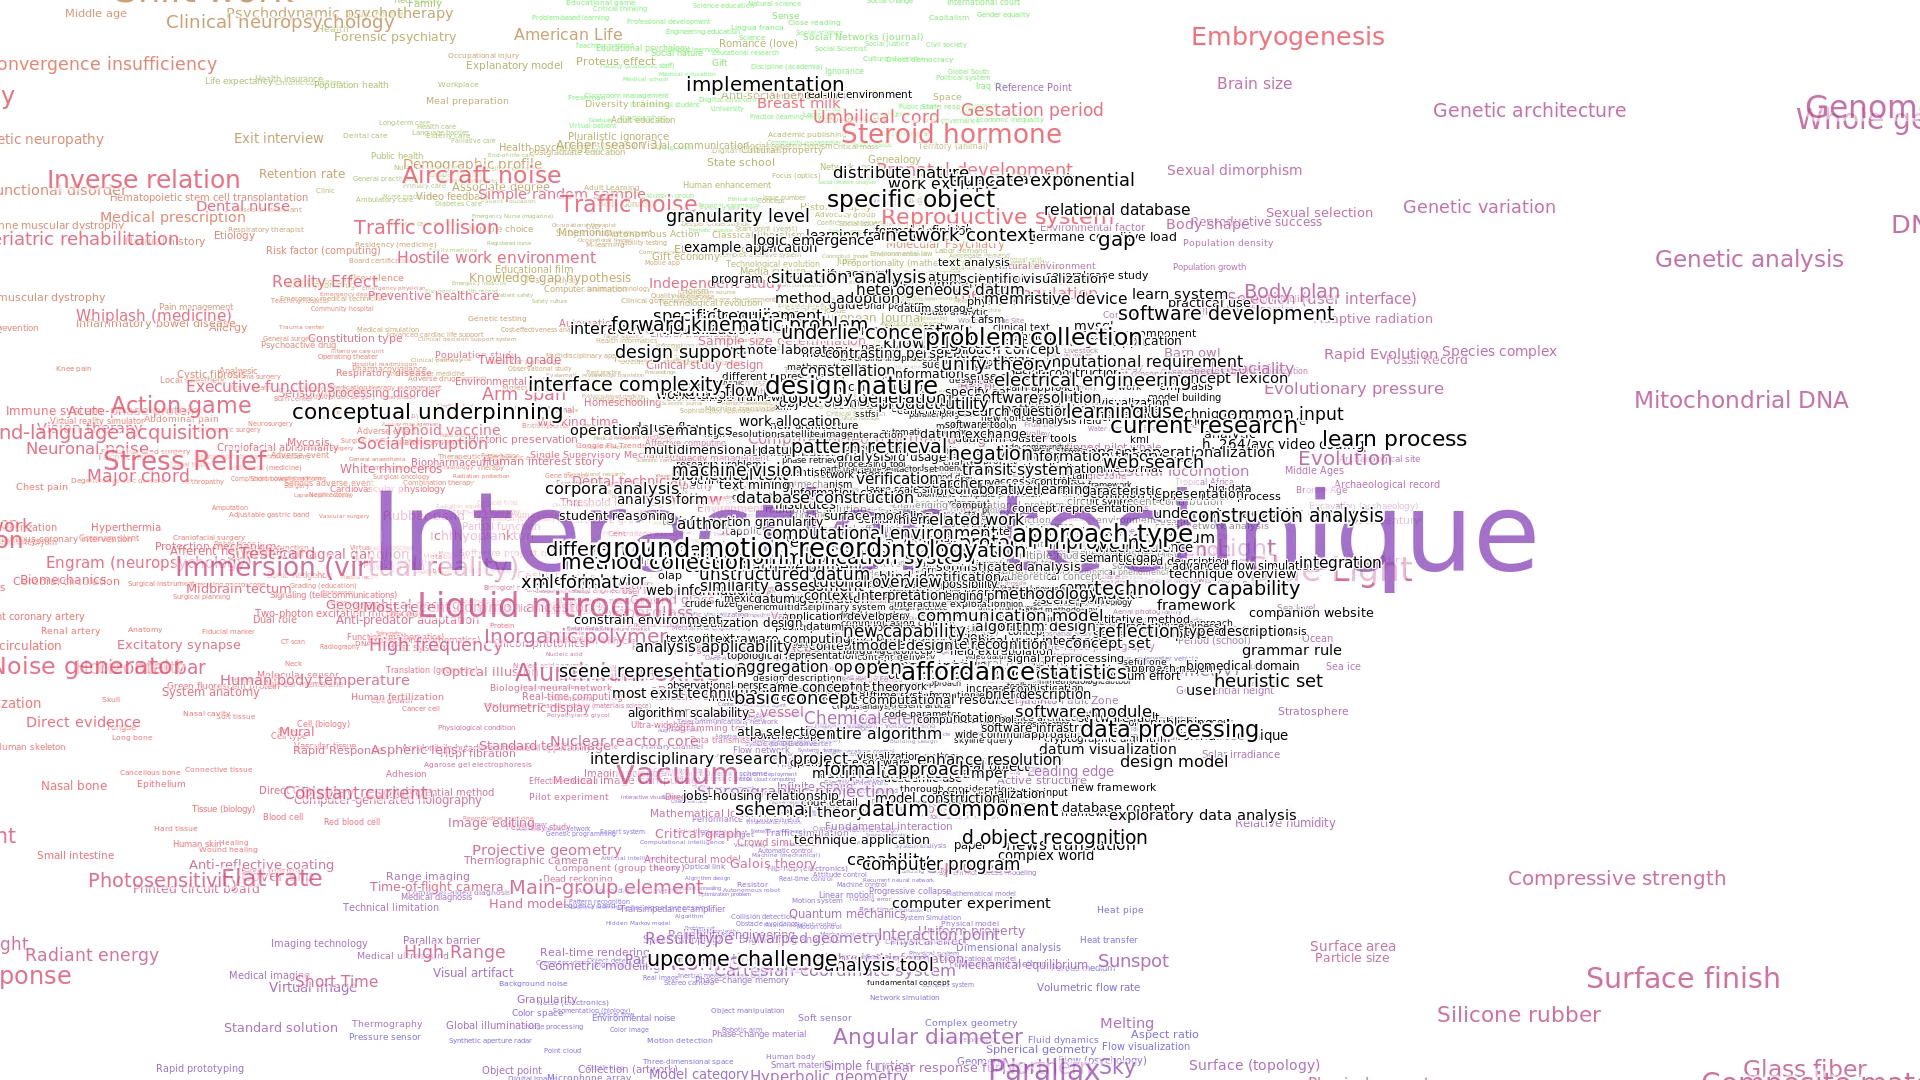
\includegraphics[width=\textwidth]{shots/local.png}
  \caption{Облако слов word2vec, находящихся в окрестности одного из слов выборки.}
\end{figure}

\begin{figure}[h]
  \centering
  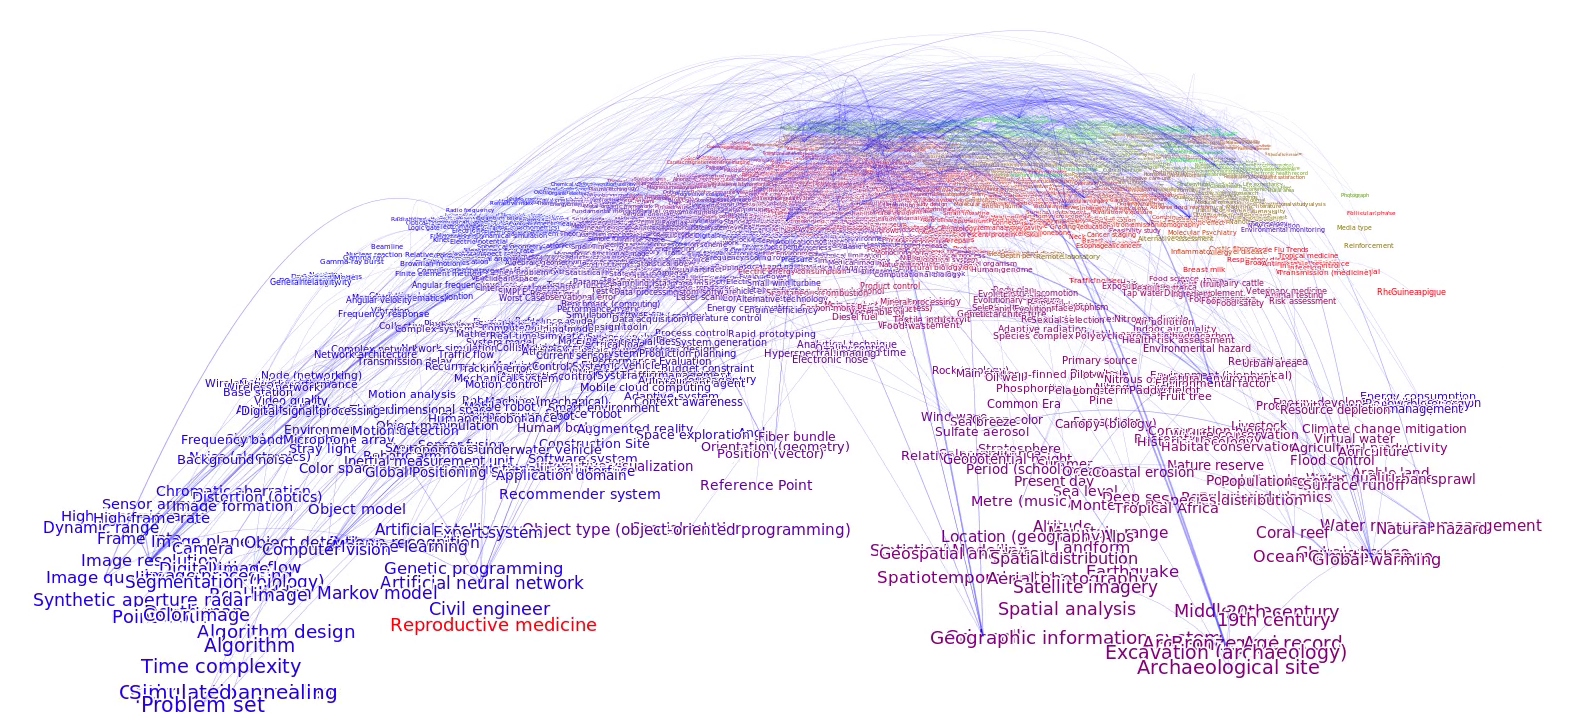
\includegraphics[width=\textwidth]{shots/3dgraph.png}
  \caption{Плоская визуализация с ребрами в виде трехмерных дуг.}
\end{figure}

\begin{figure}[h]
  \centering
  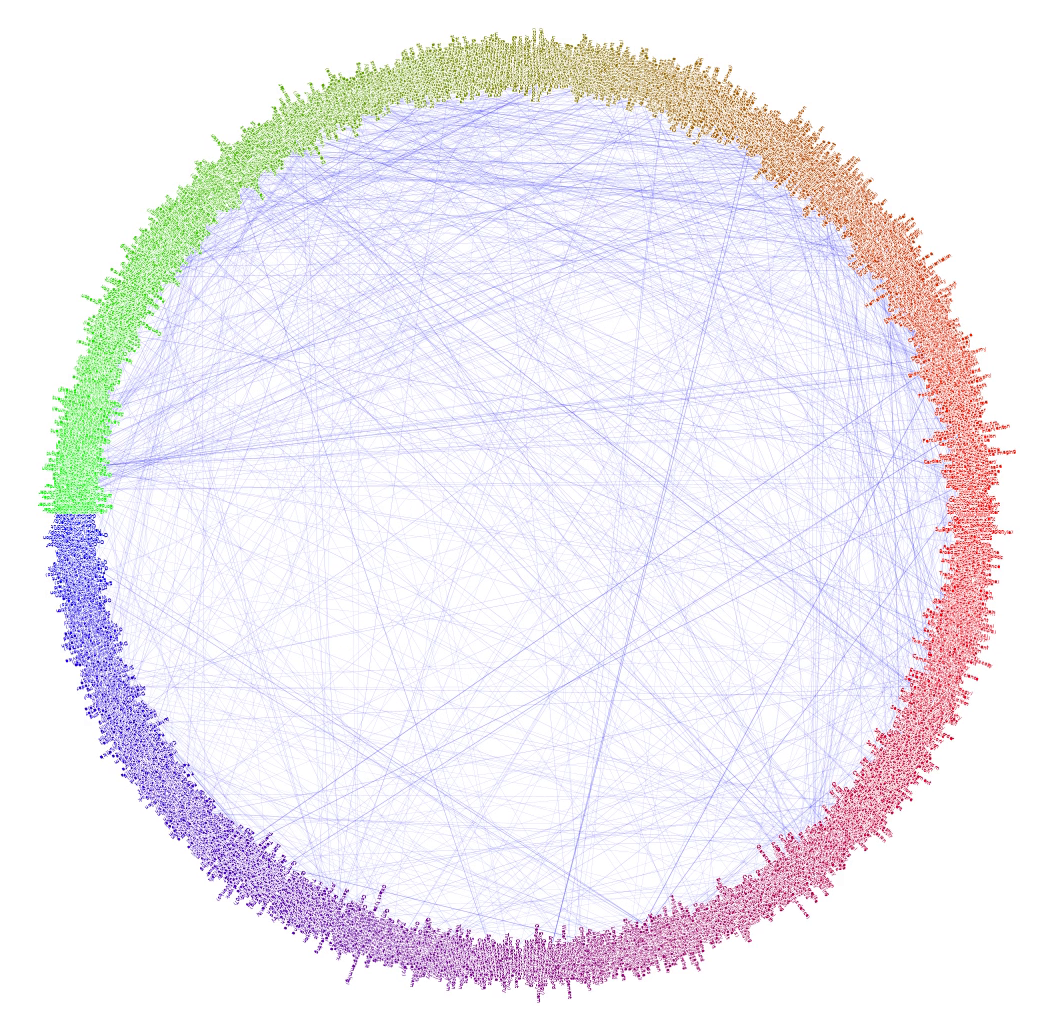
\includegraphics[width=\textwidth]{shots/circle.png}
  \caption{Пример двумерной визуализации.}
\end{figure}


\begin{figure}[h]
  \centering
  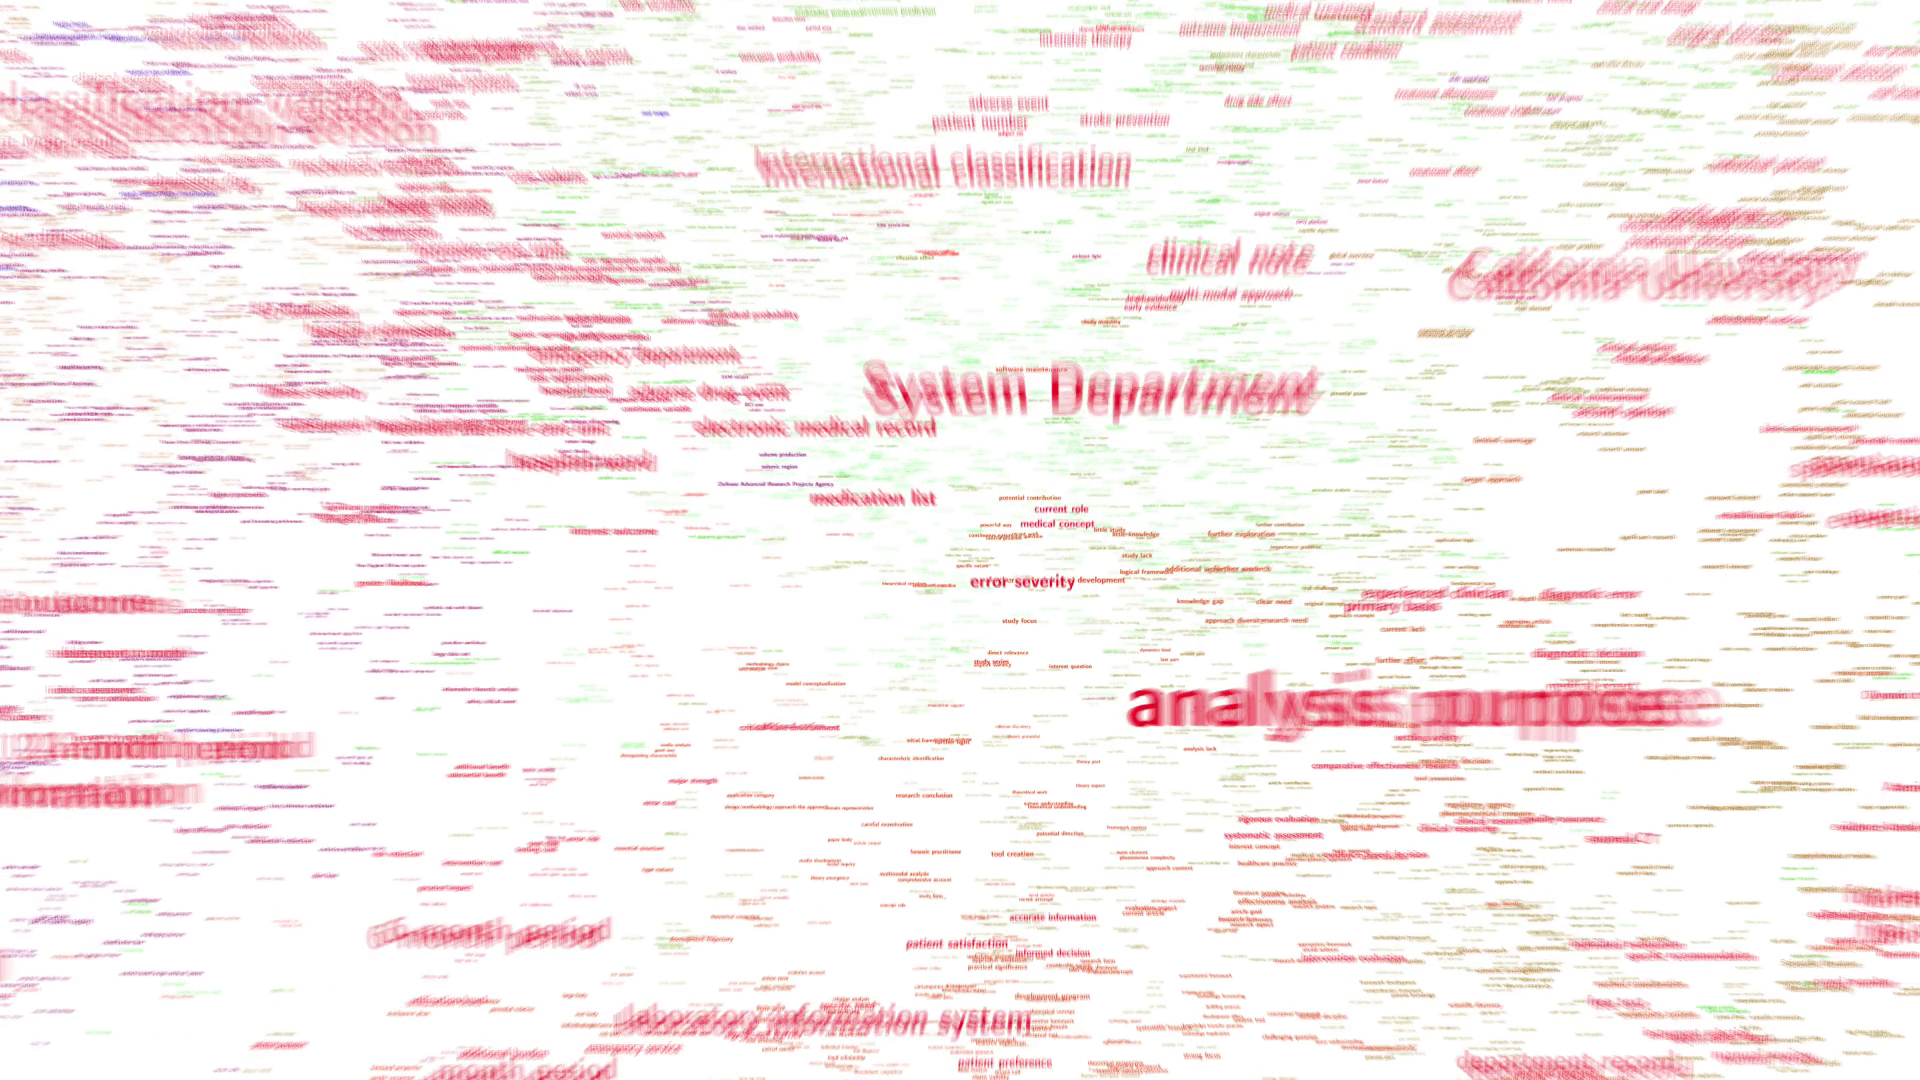
\includegraphics[width=\textwidth]{shots/motion.png}
  \caption{Пример motion blur.}
\end{figure}

\begin{figure}[h]
  \centering
  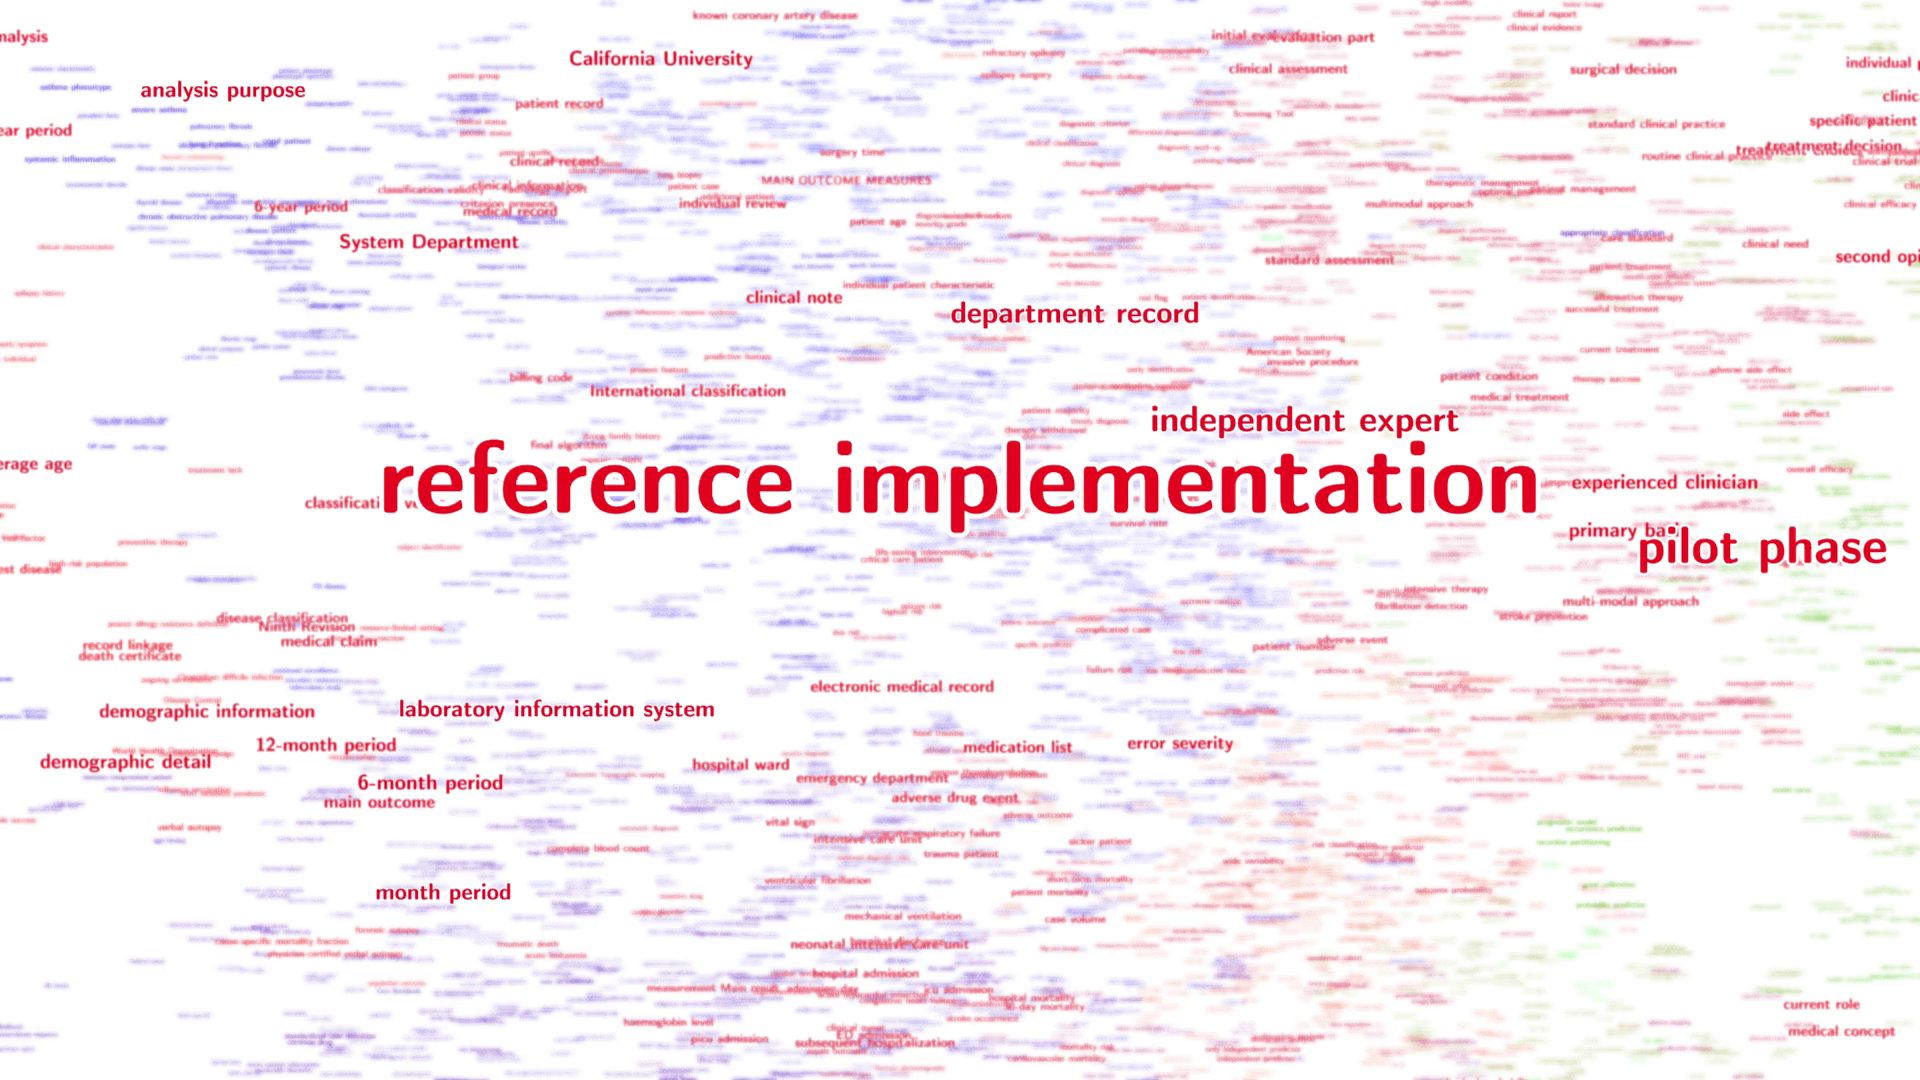
\includegraphics[width=\textwidth]{shots/lens.png}
  \caption{Пример lens blur.}
\end{figure}

\begin{figure}[h]
  \centering
  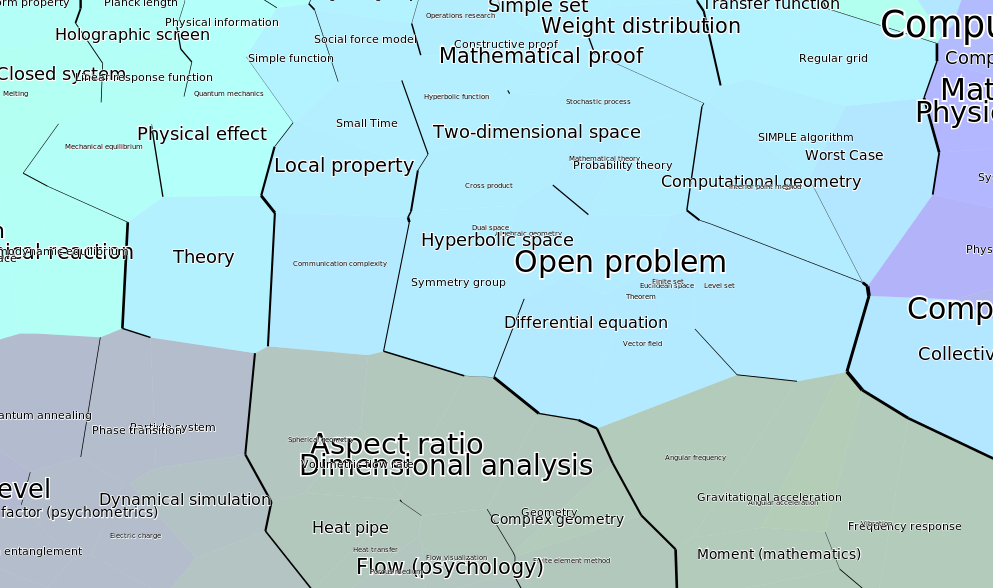
\includegraphics[width=\textwidth]{shots/voronoi_1.png}
  \caption{Пример двумерной t-SNE визуализации, дополненной информацией об искажении расстояний при помощи разной толщины границ клеток диаграммы Вороного.}
\end{figure}

\begin{figure}[h]
  \centering
  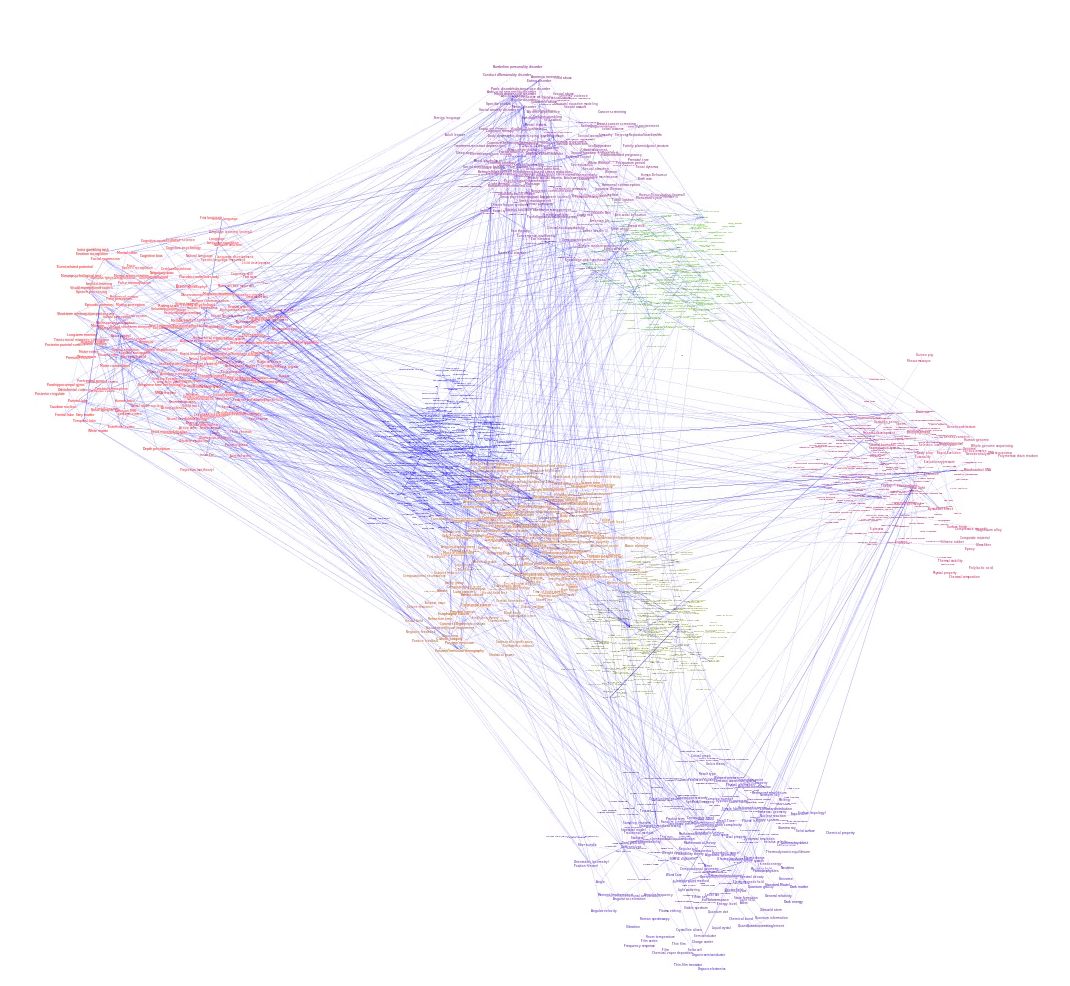
\includegraphics[width=\textwidth]{shots/clusters.png}
  \caption{Выделение K-Means кластеров вместе с ребрами.}
\end{figure}

\end{document}
  
